\chapter{Điều khiển pha thích nghi (APC)}

\section{Nguyên lý thiết kế và kiến trúc}

Bộ điều khiển pha thích nghi (Adaptive Phase Controller - APC) được thiết kế theo nguyên lý điều khiển phân tán với khả năng tự quyết định cục bộ cho từng nút giao thông. Kiến trúc này cho phép mỗi nút giao hoạt động độc lập trong khi vẫn có thể phối hợp với các nút lân cận thông qua cơ chế trao đổi thông tin. APC kết hợp giữa điều khiển dựa trên luật (rule-based control) để đảm bảo an toàn và điều khiển thích ứng (adaptive control) để tối ưu hiệu suất.

\begin{figure}[H]
    \centering
    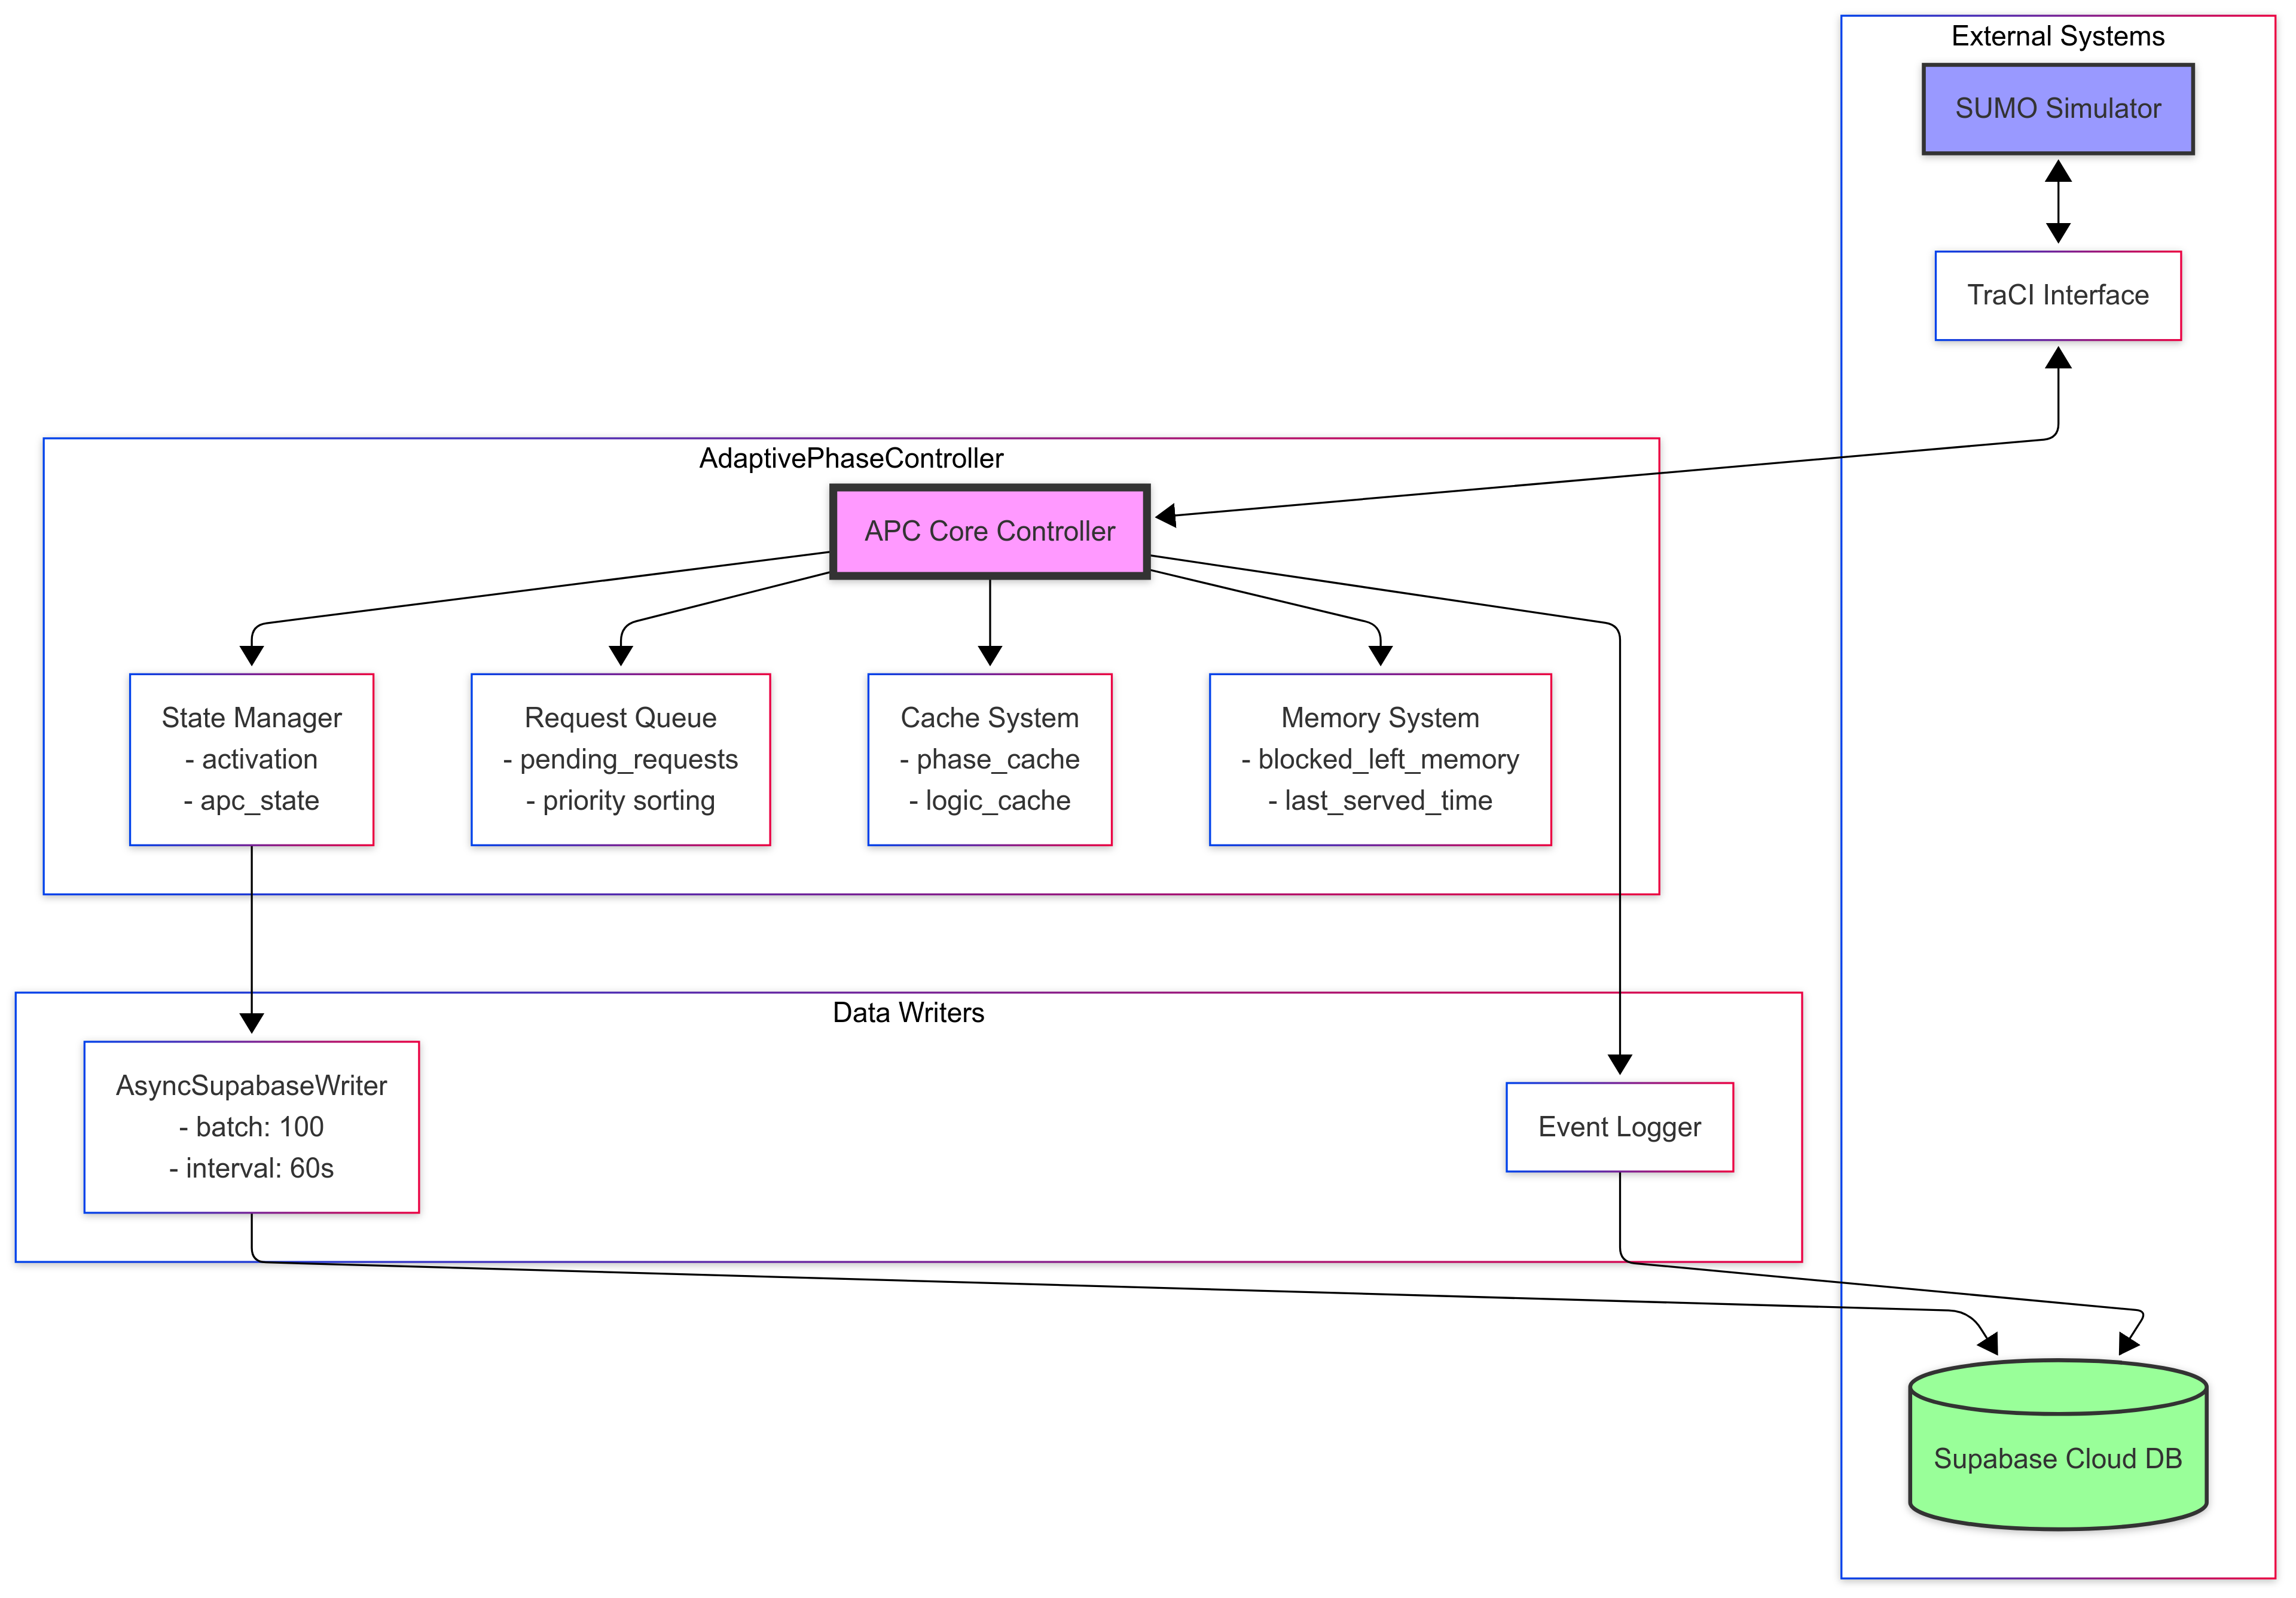
\includegraphics[width=0.9\textwidth]{Untitled diagram _ Mermaid Chart-2025-08-21-074754.png}
    \caption{Kiến trúc tổng thể của bộ điều khiển APC với các thành phần chính và luồng dữ liệu}
    \label{fig:apc_architecture}
\end{figure}
\subsection{Bộ điều khiển pha thích nghi (APC)}

AdaptivePhaseController là thành phần cốt lõi thực hiện điều khiển tín hiệu cho từng nút giao, đảm bảo hệ thống vừa an toàn vừa thích ứng linh hoạt với trạng thái giao thông thực tế. Các chức năng chính của APC gồm:

\begin{itemize}
    \item \textbf{Điều chỉnh thời lượng pha động:} APC sử dụng hàm \texttt{adjust\_phase\_duration()} để tính toán và cập nhật thời lượng pha tối ưu dựa trên các chỉ số như hàng chờ, thời gian chờ, mật độ giao thông. Công thức điều chỉnh cơ bản:
    \[
    \Delta t = \alpha \cdot (R - R_{target})
    \]
    trong đó $R$ là phần thưởng hiện tại, $R_{target}$ là mục tiêu phần thưởng động, và $\alpha$ là hệ số học. Cơ chế này giúp pha đèn tự động kéo dài hoặc rút ngắn phù hợp với nhu cầu thực tế.

    \item \textbf{Quản lý pha đèn vàng an toàn:} Hàm \texttt{insert\_yellow\_phase\_if\_needed()} tự động nhận diện và chèn pha vàng khi phát hiện chuyển đổi từ xanh sang đỏ cho bất kỳ hướng nào, đảm bảo phương tiện giảm tốc an toàn. Thời lượng pha vàng được tùy chỉnh theo tốc độ xe và chiều dài hàng chờ.

    \item \textbf{Xử lý rẽ trái bảo vệ thông minh:} Module \texttt{detect\_blocked\_left\_turn\_with\_conflict()} liên tục kiểm tra trạng thái các làn rẽ trái. Khi phát hiện bị chặn (blocked) hoặc xung đột, APC sẽ kích hoạt hoặc tạo pha rẽ trái bảo vệ riêng biệt, đảm bảo luồng giao thông không bị gián đoạn.

    \item \textbf{Quản lý yêu cầu ưu tiên:} Hệ thống hàng đợi \texttt{pending\_requests} giúp APC xử lý các yêu cầu chuyển pha theo mức độ ưu tiên rõ ràng, gồm: emergency, critical starvation, heavy congestion, và normal. Nhờ đó, các tình huống khẩn cấp, tắc nghẽn cục bộ, hoặc các hướng bị bỏ qua lâu sẽ được phục vụ kịp thời và hợp lý.
\end{itemize}
\subsection{Khởi tạo và cấu hình hệ thống}

Quá trình khởi tạo APC được thực hiện qua constructor với các tham số quan trọng:

\begin{lstlisting}[style=py, caption={Khởi tạo AdaptivePhaseController}]
def __init__(self, lane_ids, tls_id, alpha=1.0, 
             min_green=30, max_green=80,
             r_base=0.5, r_adjust=0.1, 
             severe_congestion_threshold=0.8,
             large_delta_t=20):
    self.lane_ids = lane_ids
    self.tls_id = tls_id
    # Dang ky subscription voi TraCI
    for lid in self.lane_ids:
        traci.lane.subscribe(lid, [
            traci.constants.LAST_STEP_VEHICLE_HALTING_NUMBER,
            traci.constants.LAST_STEP_MEAN_SPEED,
            traci.constants.LAST_STEP_VEHICLE_NUMBER,
            traci.constants.LAST_STEP_VEHICLE_ID_LIST,
        ])
\end{lstlisting}

\textbf{Quá trình khởi tạo bao gồm các bước chính:}

\begin{enumerate}
    \item \textbf{Thiết lập subscription với TraCI:} Hệ thống đăng ký theo dõi các metrics quan trọng cho từng làn đường được quản lý, bao gồm số lượng xe dừng, tốc độ trung bình, tổng số xe và danh sách ID phương tiện. Cơ chế subscription giúp tối ưu băng thông bằng cách chỉ nhận dữ liệu cần thiết.
    
    \item \textbf{Khởi tạo cấu trúc dữ liệu:} Các container quan trọng được khởi tạo:
    \begin{itemize}
        \item \texttt{apc\_state}: Dictionary lưu trữ trạng thái toàn cục với events queue (maxlen=5000) và danh sách phases
        \item \texttt{pending\_requests}: Hàng đợi yêu cầu chuyển pha với cơ chế ưu tiên
        \item \texttt{phase\_cache}: Cache thông tin pha với TTL 30 giây để giảm truy vấn database
        \item \texttt{blocked\_left\_memory}: Dictionary theo dõi lịch sử làn rẽ trái bị chặn
    \end{itemize}
    
    \item \textbf{Kết nối database:} Khởi tạo \texttt{PatchedAsyncSupabaseWriter} với interval 60 giây và batch size 100 records để đồng bộ dữ liệu không đồng bộ lên cloud.
    
    \item \textbf{Tải trạng thái từ Supabase:} Phương thức \texttt{\_load\_apc\_state\_supabase()} được gọi để khôi phục trạng thái từ lần chạy trước, đảm bảo tính liên tục của hệ thống.
    
    \item \textbf{Đồng bộ pha với SUMO:} \texttt{preload\_phases\_from\_sumo()} đảm bảo tất cả các pha trong logic đèn được ghi nhận và có base duration phù hợp.
\end{enumerate}
\begin{figure}[H]
    \centering
    \begin{subfigure}[b]{0.65\textwidth}
        \centering
        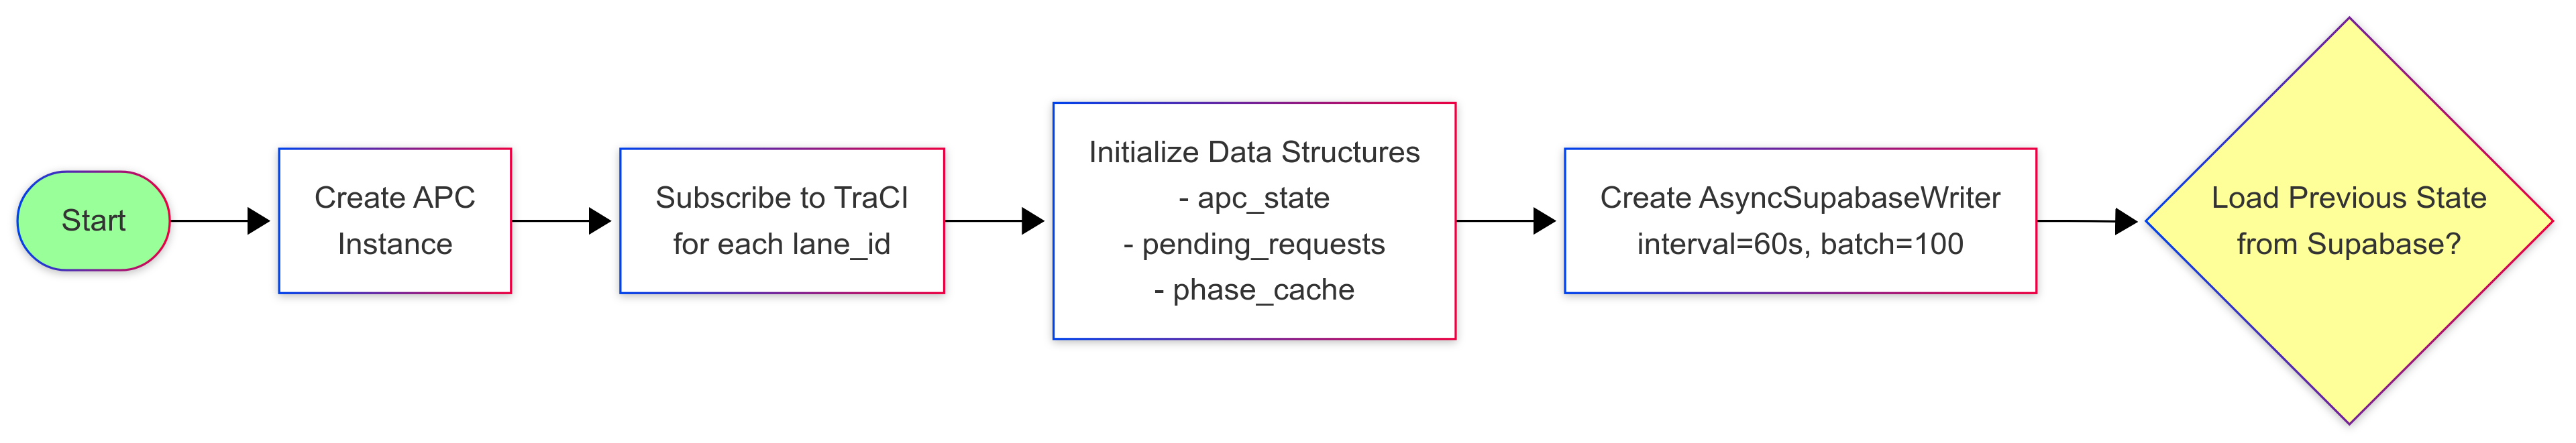
\includegraphics[width=1.1\textwidth]{Untitled diagram _ Mermaid Chart-2025-08-21-084042.png}
        \caption{Khởi tạo và thiết lập}
    \end{subfigure}
    \hfill
    \begin{subfigure}[b]{0.65\textwidth}
        \centering
        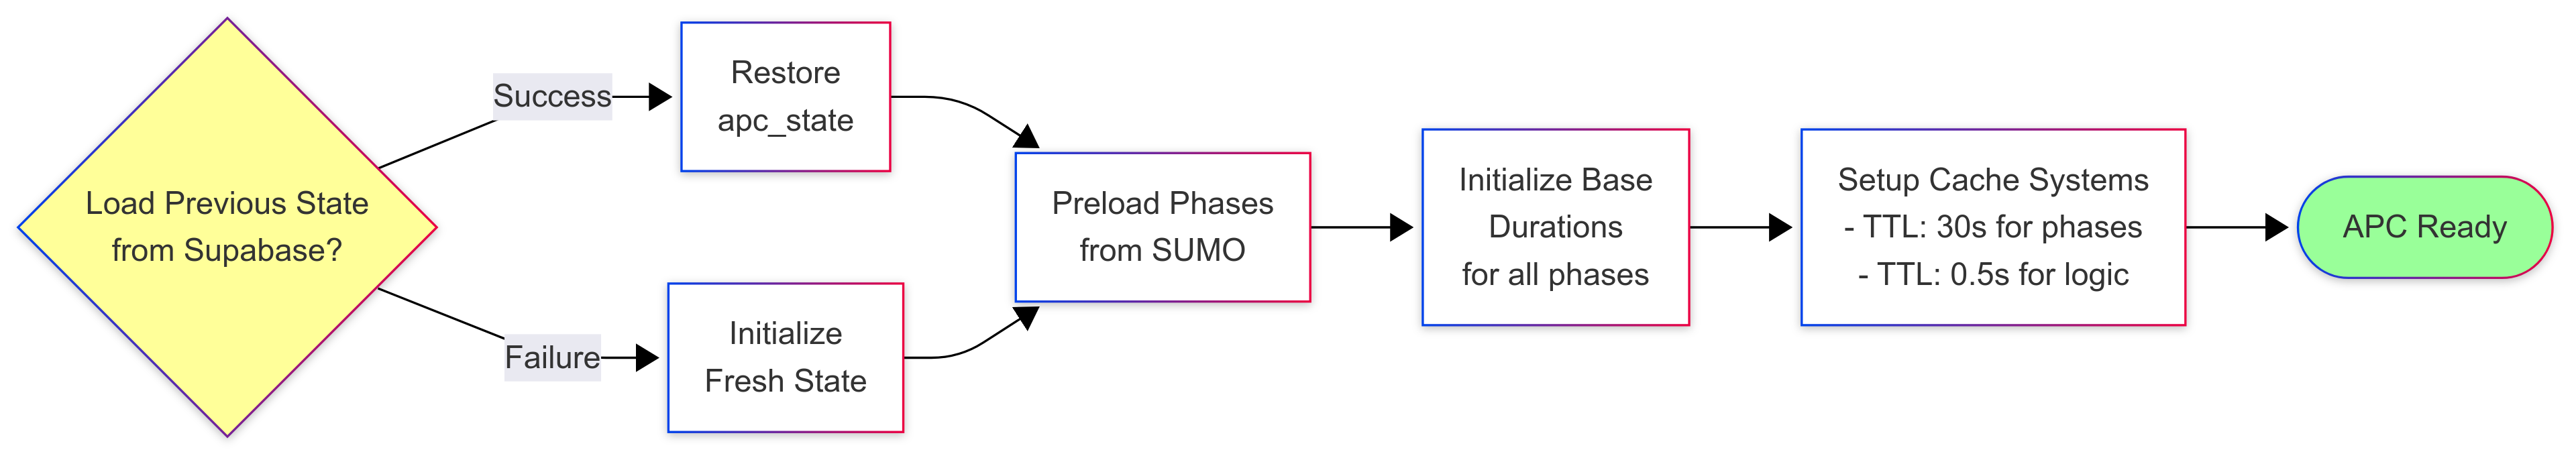
\includegraphics[width=1.1\textwidth]{Untitled diagram _ Mermaid Chart-2025-08-21-084132.png}
        \caption{Khôi phục trạng thái và hoàn tất}
    \end{subfigure}
    \caption{Quy trình khởi tạo AdaptivePhaseController.}
    \label{fig:apc_init_flow}
\end{figure}
\subsection{Cấu trúc dữ liệu và tham số điều khiển}

APC sử dụng hệ thống tham số phân cấp để điều chỉnh hành vi:

\subsubsection{Tham số thời gian}
\begin{itemize}
    \item \texttt{min\_green} (mặc định 30s): Thời gian tối thiểu cho mỗi pha xanh, đảm bảo an toàn và công bằng
    \item \texttt{max\_green} (mặc định 80s): Giới hạn trên để tránh độc quyền một hướng
    \item \texttt{low\_demand\_extend\_cap} (4s): Giới hạn mở rộng khi nhu cầu (lượng xe) thấp
\end{itemize}

\subsubsection{Tham số điều khiển thích ứng}
\begin{itemize}
    \item \texttt{alpha} (1.0): Hệ số học trong công thức điều chỉnh $\Delta t = \alpha(R - R_{target})$
    \item \texttt{r\_base} (0.5): Giá trị reward cơ sở cho thuật toán học
    \item \texttt{r\_adjust} (0.1): Hệ số điều chỉnh R\_target động
    \item \texttt{weights} (vector 4D): Trọng số cho [density, speed, wait, queue] trong hàm reward
\end{itemize}

\paragraph{Cập nhật mục tiêu reward động (\(R_{target}\)):}
Để hệ thống APC thích nghi tốt với trạng thái giao thông thực tế, giá trị mục tiêu reward (\(R_{target}\)) được điều chỉnh động dựa trên reward trung bình gần nhất. Công thức tính như sau:

\[
R_{target} = r_{base} + r_{adjust} \cdot (\overline{R} - r_{base})
\]

Trong đó:
\begin{itemize}
    \item \(r_{base}\): Giá trị reward cơ sở, phản ánh mức hiệu suất tối thiểu kỳ vọng.
    \item \(r_{adjust}\): Hệ số điều chỉnh, kiểm soát mức độ nhạy của mục tiêu với trạng thái thực tế.
    \item \(\overline{R}\): Giá trị reward trung bình gần nhất (ví dụ: trung bình cộng của reward trong một cửa sổ thời gian hoặc số chu kỳ trước).
\end{itemize}

Việc cập nhật \(R_{target}\) giúp APC tự động thích ứng khi điều kiện giao thông thay đổi (ví dụ: tắc nghẽn, lưu lượng tăng đột biến), từ đó tối ưu hóa quá trình điều chỉnh thời lượng pha đèn.
\subsubsection{Ngưỡng phát hiện sự kiện}

\subsubsection{Cấu trúc dữ liệu chính}

\textbf{Activation State:} Dictionary theo dõi pha đang hoạt động:
\begin{lstlisting}[style=py]
self.activation = {
    "phase_idx": None,        # Chi so pha hien tai
    "start_time": 0.0,        # Thoi diem bat dau
    "base_duration": None,    # Thoi luong co so
    "desired_total": None     # Thoi luong mong muon
}
\end{lstlisting}

\textbf{Pending Requests Queue:} Danh sách các yêu cầu chuyển pha được sắp xếp theo priority và timestamp:
\begin{lstlisting}[style=py]
request = {
    "phase_idx": int,         # Pha muc tieu
    "priority": int,          # Muc uu tien (1-11)
    "priority_type": str,     # Loai: emergency, starvation...
    "extension_duration": float,  # Thoi luong yeu cau
    "timestamp": float        # Thoi diem tao yeu cau
}
\end{lstlisting}
\begin{figure}[H]
    \centering
    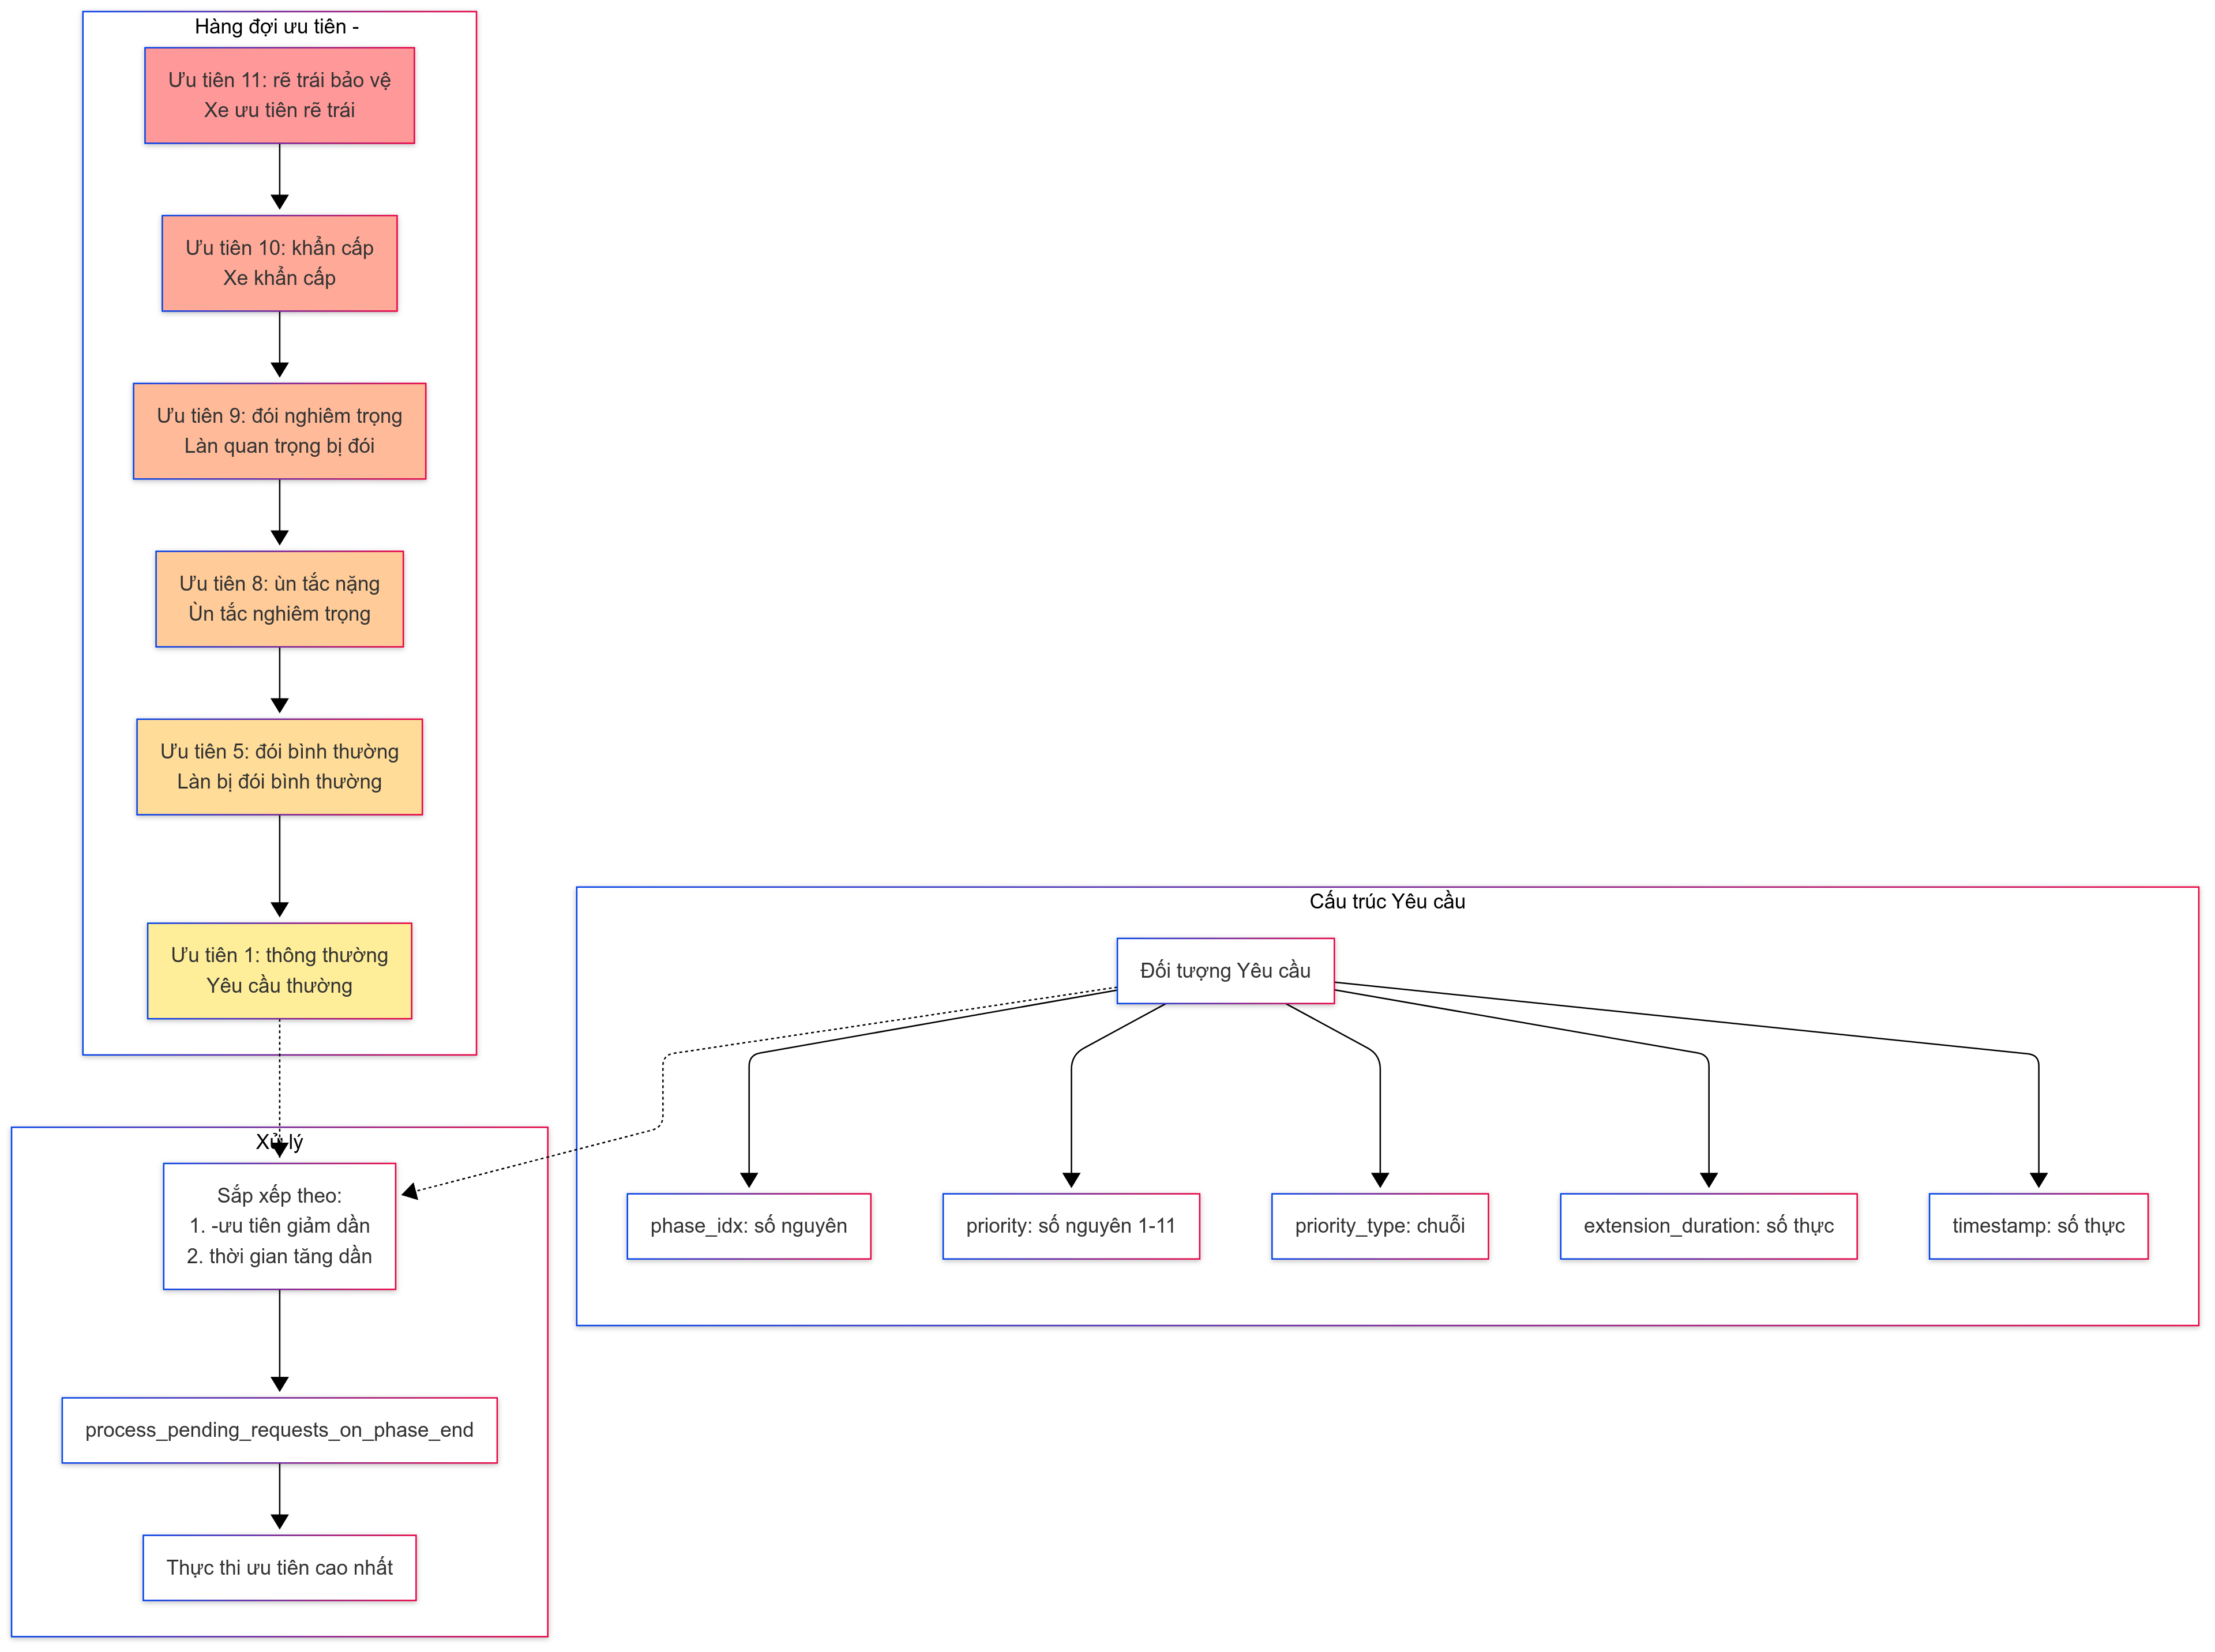
\includegraphics[width= 1.1\textwidth]{Untitled diagram _ Mermaid Chart-2025-08-22-072612.png}
    \caption{Cấu trúc hàng đợi yêu cầu với mức độ ưu tiên}
    \label{fig:priority_queue}
\end{figure}
\subsection{Tích hợp với TraCI và SUMO}

Việc tích hợp với SUMO thông qua TraCI được thực hiện qua nhiều lớp abstraction:

\subsubsection{Cơ chế Subscription}
APC sử dụng TraCI subscription để nhận dữ liệu real-time hiệu quả:

\begin{lstlisting}[style=py, caption={Xử lý subscription results}]
def get_lane_stats(self, lane_id):
    res = traci.lane.getSubscriptionResults(lane_id) or {}
    q = float(res.get(
        traci.constants.LAST_STEP_VEHICLE_HALTING_NUMBER,
        traci.lane.getLastStepHaltingNumber(lane_id)
    ))
    v = float(res.get(
        traci.constants.LAST_STEP_MEAN_SPEED,
        traci.lane.getLastStepMeanSpeed(lane_id)
    ))
    return q, w, v, dens
\end{lstlisting}

\subsubsection{Logic Cache System}
Để giảm overhead communication, APC implement cache cho traffic light logic:

\begin{lstlisting}[style=py, caption={Cơ chế cache logic}]
def _get_logic(self):
    now = traci.simulation.getTime()
    if self._logic_cache is None or \
       now - self._logic_cache_at > self._logic_cache_ttl:
        self._logic_cache = get_current_logic(self.tls_id)
        self._logic_cache_at = now
    return self._logic_cache
\end{lstlisting}

Cache có thời gian sống (TTL) là 0.5 giây và sẽ được làm mới (invalidate) khi cấu trúc pha đèn thay đổi. Ngoài ra, hệ thống còn hỗ trợ cache dùng chung ở cấp độ controller để tối ưu hiệu suất khi có nhiều bộ điều khiển APC hoạt động đồng thời.

\subsubsection{Safe Control Wrappers}
Mọi lệnh điều khiển được wrap trong các hàm an toàn:

\begin{lstlisting}[style=py, caption={Safe phase control}]
def _apply_phase(self, phase_idx, duration):
    # Clamp phase index
    safe_idx = self._safe_phase_index(phase_idx, 
                                      force_reload=True)
    if safe_idx is None:
        return False
    
    # Try controller-level setter first
    if hasattr(self, "controller"):
        ok = self.controller._safe_set_phase(
            self.tls_id, safe_idx, duration
        )
        if ok:
            return True
            
    # Fallback to direct control
    return safe_set_phase(self.tls_id, safe_idx, duration)
\end{lstlisting}

Cơ chế này đảm bảo:
\begin{itemize}
    \item Phase index luôn nằm trong giới hạn hợp lệ
    \item Duration được giới hạn trong khoảng [min\_green, max\_green]
    \item Xử lý graceful khi SUMO reject lệnh điều khiển
    \item Đồng bộ state giữa APC và SUMO
\end{itemize}
Thiết kế tích hợp này cho phép APC hoạt động ổn định trong môi trường mô phỏng phức tạp, xử lý được các trường hợp đặc biệt như chỉ số pha vượt giới hạn, thay đổi cấu trúc mạng, và lỗi kết nối với supabse.
\section{Quản lý logic pha đèn tín hiệu}

Quản lý logic pha đèn tín hiệu là thành phần cốt lõi đảm bảo hoạt động an toàn và hiệu quả của hệ thống điều khiển. APC áp dụng một hệ thống quản lý logic đa tầng với cơ chế cache thông minh, kiểm soát chuyển pha an toàn và xử lý xung đột tự động.

\subsection{Cơ chế cache và tối ưu truy xuất}

Hệ thống cache được xây dựng theo hai lớp, giúp giảm lượng truy cập tới SUMO mà vẫn giữ cho dữ liệu luôn đồng bộ và nhất quán.
\subsubsection{Cache cục bộ APC}

Mỗi bộ điều khiển APC sẽ giữ một bộ nhớ đệm (cache) riêng cho logic đèn giao thông, với thời gian tồn tại của cache là 0.5 giây (Time To Live - TTL).

\begin{lstlisting}[style=py, caption={Implementation của logic cache cục bộ}]
def _get_logic(self):
    now = traci.simulation.getTime()
    # Kiem tra cache validity
    if self._logic_cache is None or \
       now - self._logic_cache_at > self._logic_cache_ttl:
        try:
            # Fetch fresh logic tu SUMO
            self._logic_cache = get_current_logic(self.tls_id)
            self._logic_cache_at = now
        except Exception:
            self._logic_cache = None
    return self._logic_cache
\end{lstlisting}

Cache hoạt động theo nguyên tắc:
\begin{itemize}
    \item \textbf{Lazy loading}: Logic chỉ được fetch khi cần thiết
    \item \textbf{Time-based invalidation}: Tự động expire sau 0.5 giây
    \item \textbf{Explicit invalidation}: Force refresh khi có mutation
\end{itemize}
%\vspace{3cm}
\subsubsection{Shared cache ở Controller level}
Khi nhiều APC cùng hoạt động, hệ thống sử dụng shared cache để tối ưu:

\begin{lstlisting}[style=py, caption={Shared cache mechanism (chỉ với tls\_id: E3)}]
def _get_logic(self):
    controller = getattr(self, "controller", None)
    if controller and hasattr(controller, "tl_logic_cache"):
        entry = controller.tl_logic_cache.get(self.tls_id)
        if entry and (now - entry.get("at", -1)) <= self._logic_cache_ttl:
            return entry.get("logic")
        # Update shared cache
        logic = get_current_logic(self.tls_id)
        controller.tl_logic_cache[self.tls_id] = {
            "logic": logic, 
            "at": now
        }
        return logic
\end{lstlisting}

\vspace{1cm}

\begin{figure}[H]
    \centering
    % Chỉ thể hiện APC Instance với tls_id: E3
    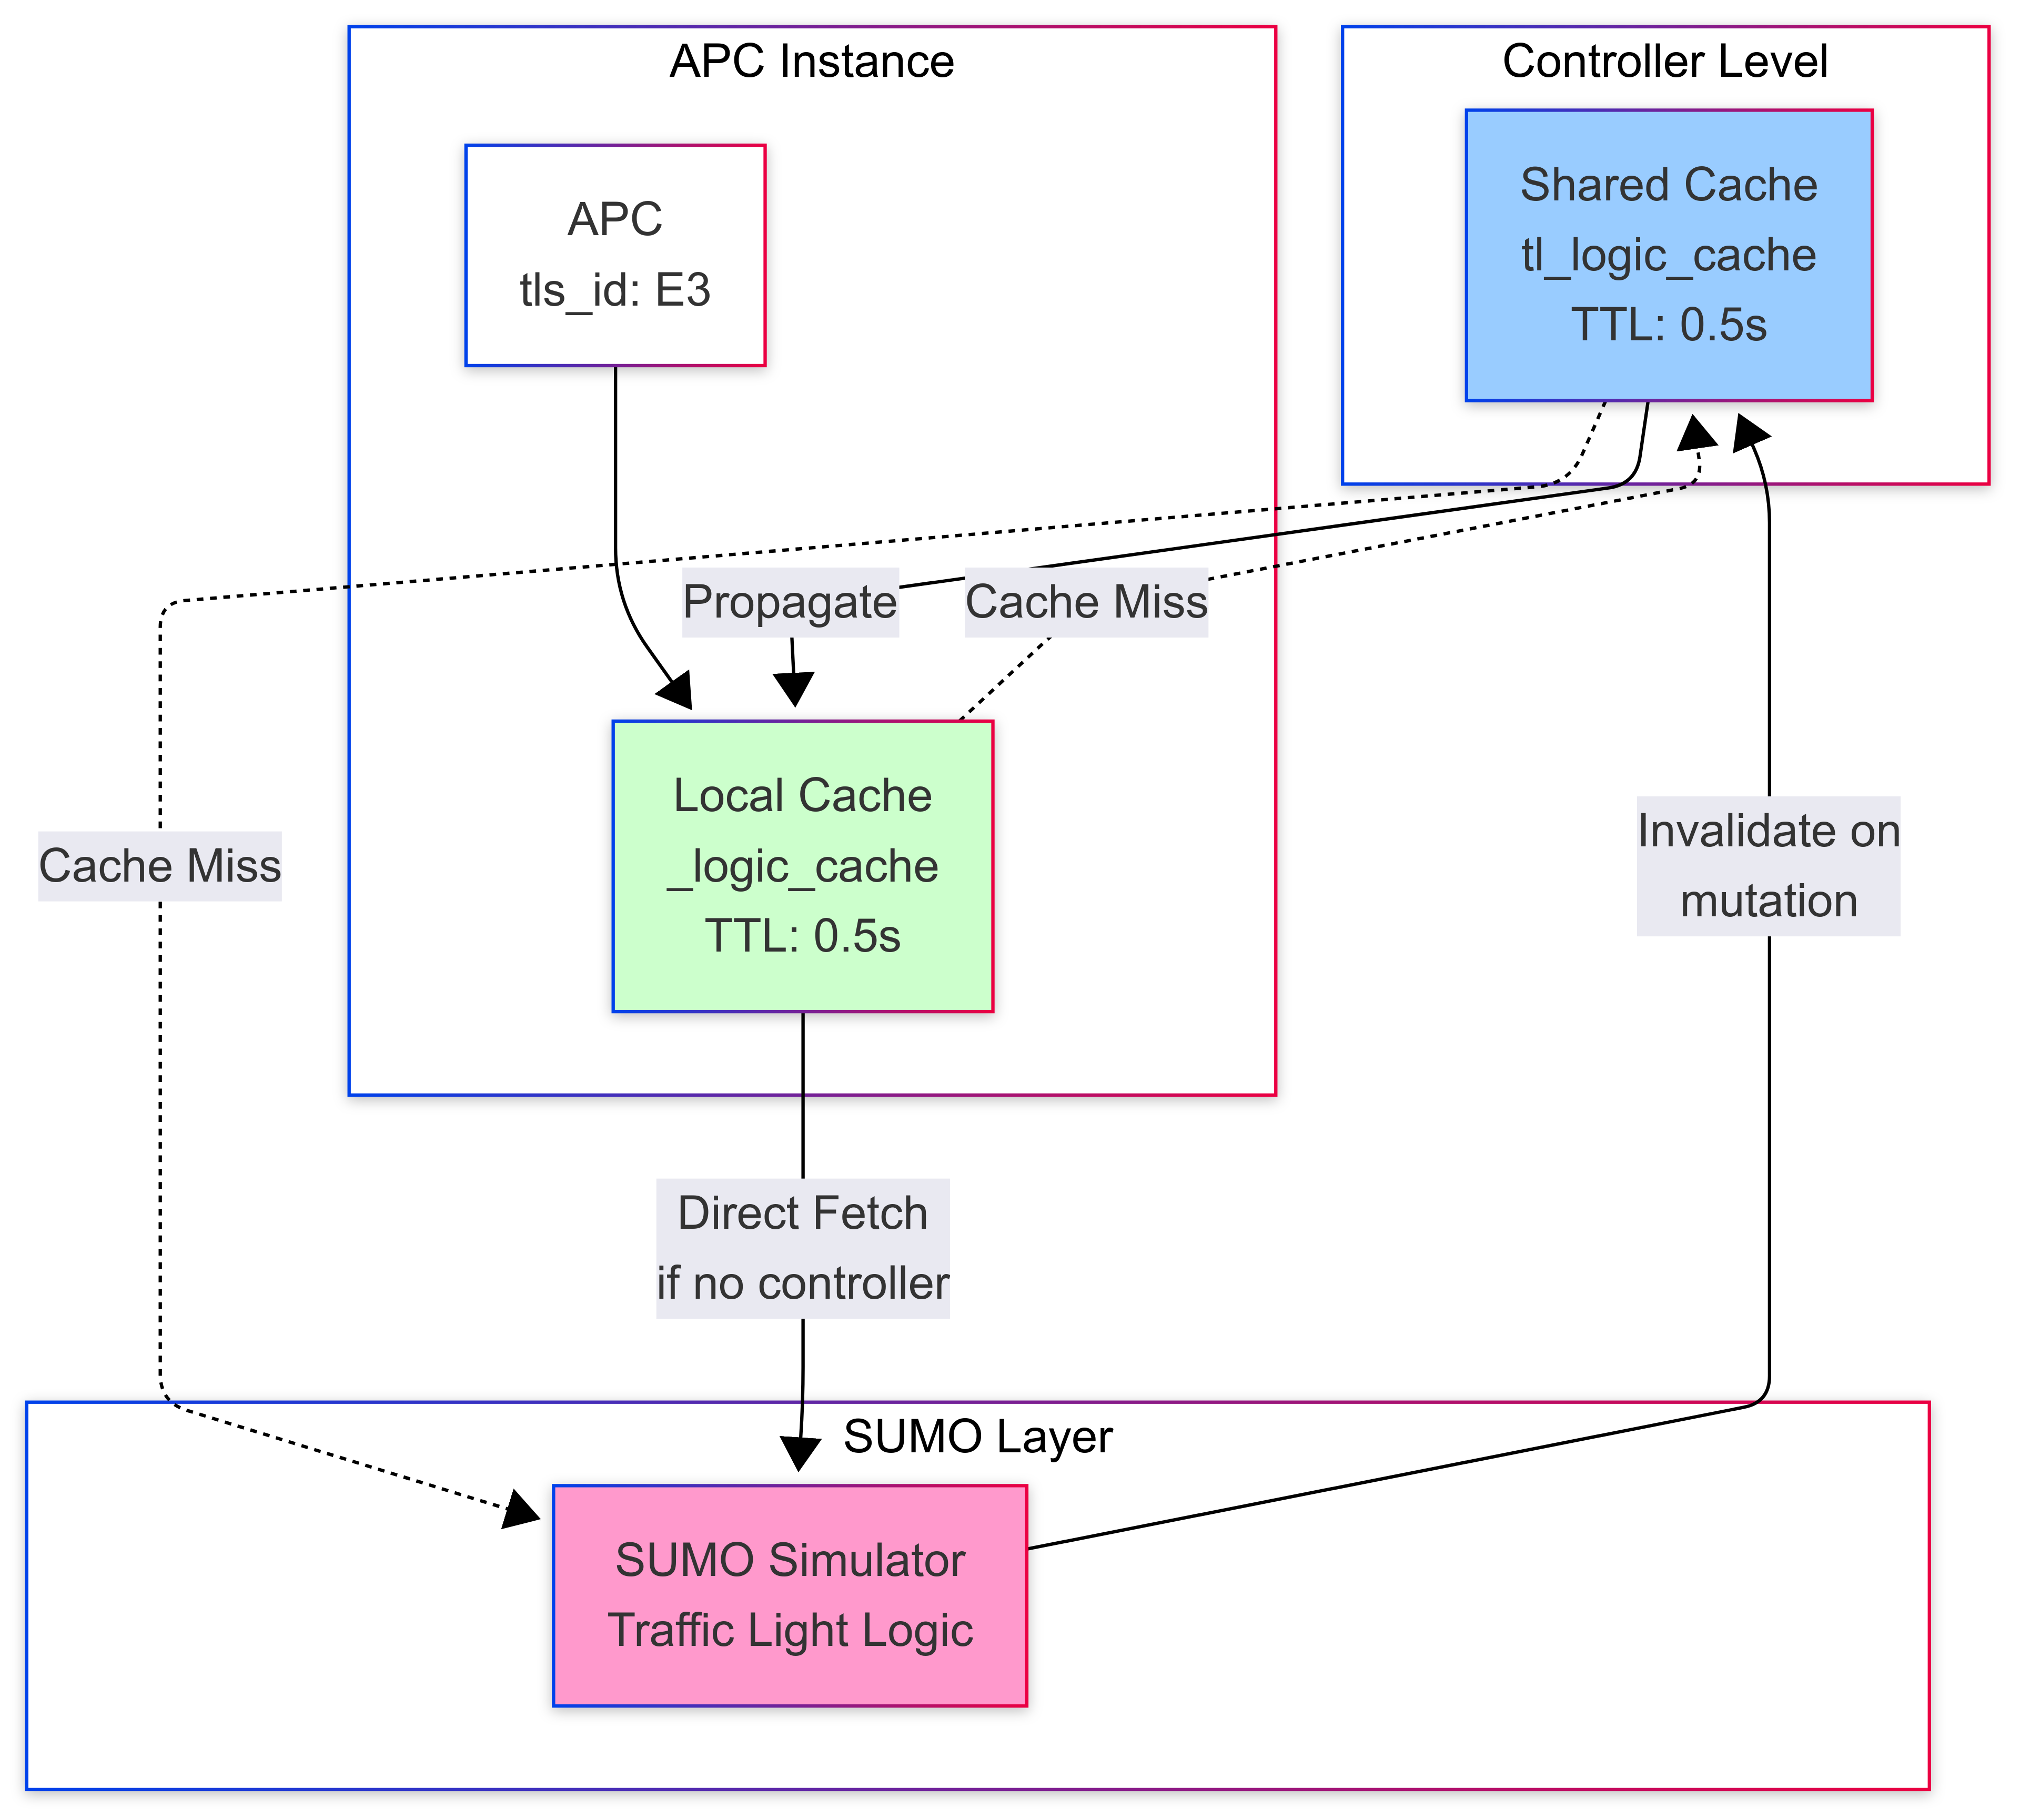
\includegraphics[width=0.85\linewidth]{Untitled diagram _ Mermaid Chart-2025-08-22-044929.png}
    \caption{Kiến trúc cache hai tầng cho traffic light logic chỉ với APC: E3}
    \label{fig:cache_architecture}
\end{figure}

\subsubsection{Cache invalidation strategy}

Hệ thống sử dụng cơ chế xóa (invalidation) thông minh để luôn duy trì sự nhất quán dữ liệu.

\begin{lstlisting}[style=py, caption={Cache invalidation mechanism}]
def _invalidate_logic_cache(self, tl_id=None):
    # Invalidate local cache
    self._logic_cache = None
    self._logic_cache_at = -1.0
    
    # Propagate to controller level
    controller = getattr(self, "controller", None)
    if controller and hasattr(controller, "_invalidate_logic_cache"):
        controller._invalidate_logic_cache(self.tls_id)
\end{lstlisting}
Cache sẽ bị xóa và làm mới trong các trường hợp sau:

\begin{enumerate}
    \item Khi có thao tác thêm, xóa hoặc chỉnh sửa pha đèn tín hiệu.
    \item Khi phát hiện dữ liệu không đồng nhất với trạng thái thực tế từ SUMO.
    \item Khi cấu trúc mạng lưới giao thông bị thay đổi.
\end{enumerate}

\subsection{Điều khiển chuyển pha an toàn}

Việc chuyển pha được thực hiện qua nhiều lớp kiểm tra an toàn để đảm bảo không vi phạm ràng buộc và tránh xung đột.

\subsubsection{Kiểm tra chỉ số pha hợp lệ}

Trước khi thực hiện chuyển pha đèn, hệ thống sẽ kiểm tra để đảm bảo chỉ số pha nằm trong phạm vi cho phép.

\begin{lstlisting}[style=py, caption={kẹp chỉ số pha hợp lệ}]
def _safe_phase_index(self, idx, force_reload=False):
    try:
        if force_reload:
            self._invalidate_logic_cache()
        logic = self._get_logic()
        if not logic or len(logic.getPhases()) <= 0:
            return None
        n = len(logic.getPhases())
        # Clamp to valid range
        return max(0, min(idx, n - 1))
    except Exception:
        return None
\end{lstlisting}

\subsubsection{Áp dụng pha theo nhiều tầng:}

Hệ thống thực hiện chuyển pha theo từng lớp kiểm tra và dự phòng, đảm bảo nếu một cách chuyển pha không thành công thì sẽ thử các phương án khác tiếp theo.
\begin{lstlisting}[style=py, caption={Quy trình áp dụng pha theo cấu trúc phân tầng}]
def _apply_phase(self, phase_idx, duration):
    # Layer 1: Validate and clamp
    safe_idx = self._safe_phase_index(phase_idx, force_reload=True)
    if safe_idx is None:
        return False
    
    # Layer 2: Try controller-level setter
    controller = getattr(self, "controller", None)
    if controller:
        ok = controller._safe_set_phase(
            self.tls_id, safe_idx, duration
        )
        if ok:
            return True
    
    # Layer 3: Direct SUMO control
    ok2 = safe_set_phase(self.tls_id, safe_idx, duration)
    return ok2
\end{lstlisting}

\begin{figure}[htbp]
    \centering
    \begin{minipage}[t]{0.48\textwidth}
        \centering
        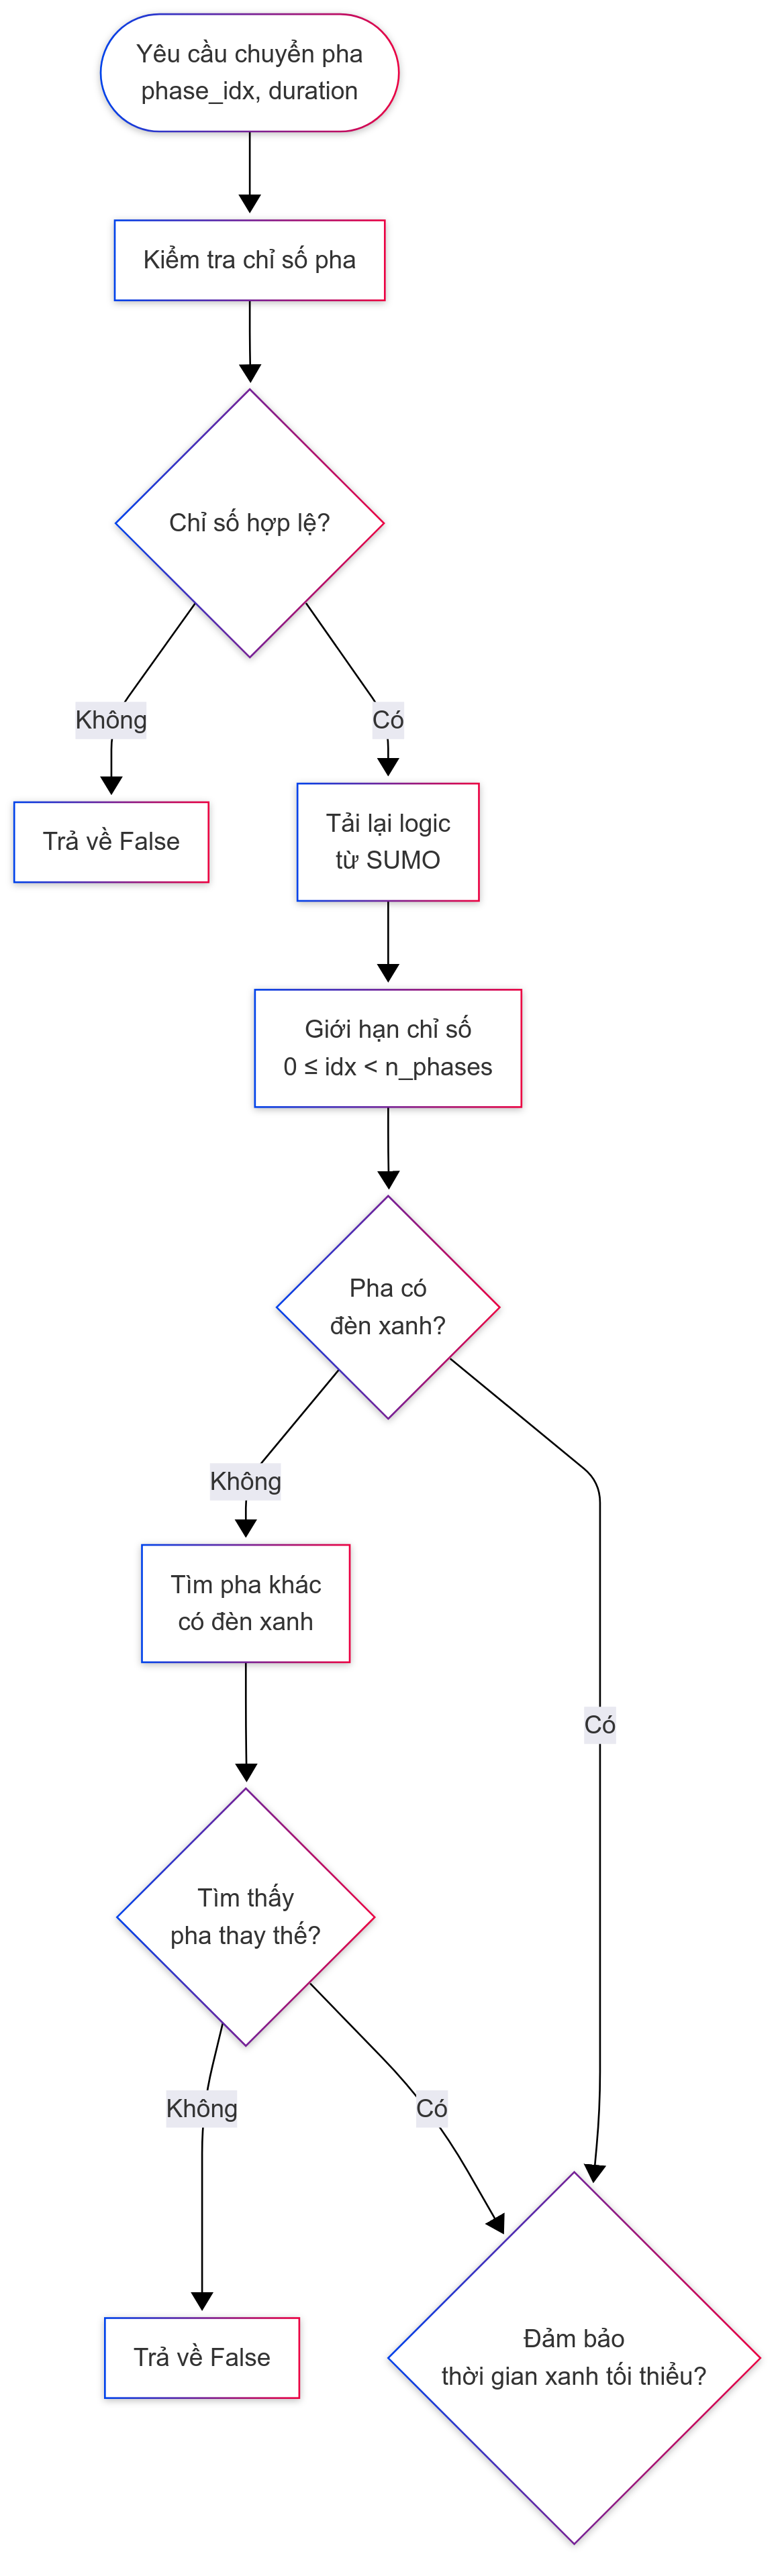
\includegraphics[width=0.9\linewidth]{Untitled diagram _ Mermaid Chart-2025-08-22-064822.png}
        \caption*{(a) Kiểm tra \& xác thực chỉ số pha}
    \end{minipage}
    \hfill
    \begin{minipage}[t]{0.48\textwidth}
        \centering
        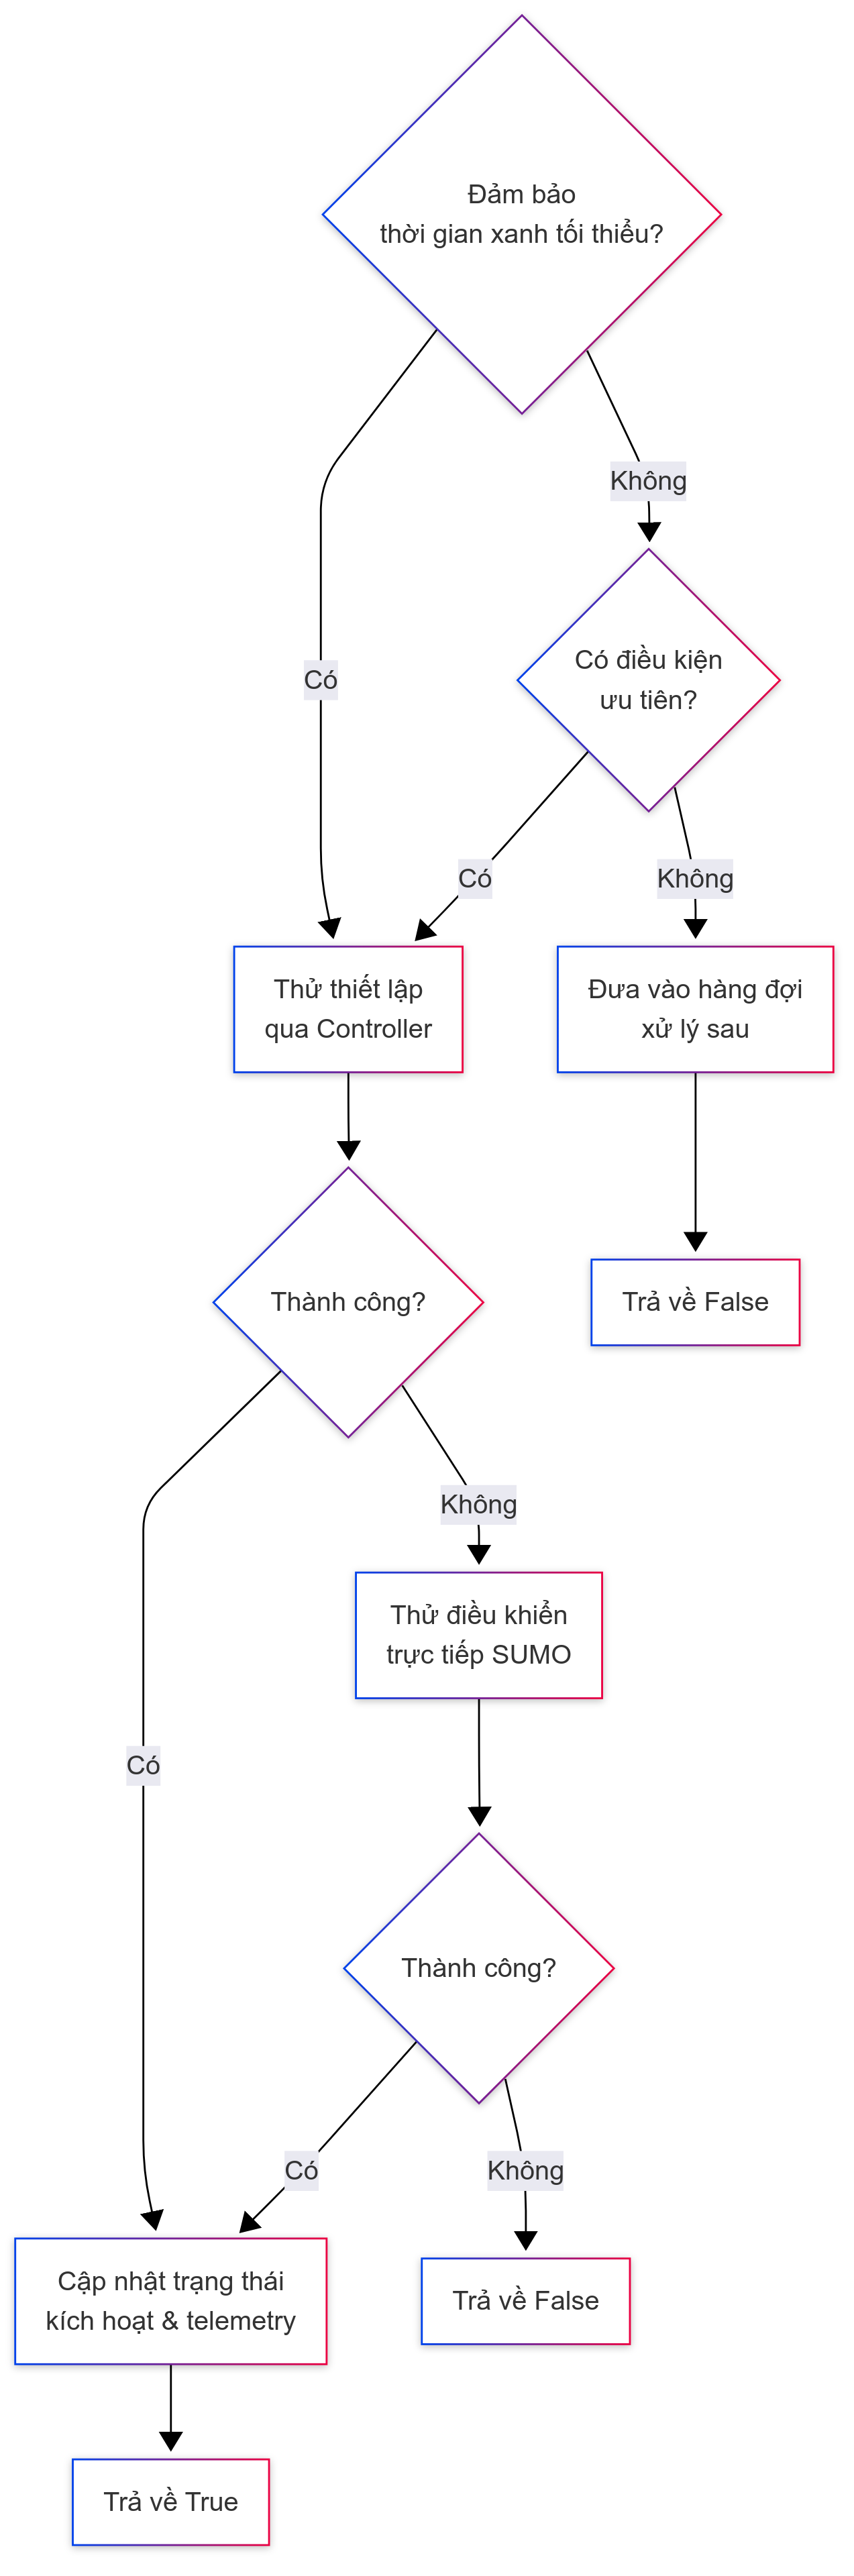
\includegraphics[width=0.9\linewidth]{Untitled diagram _ Mermaid Chart-2025-08-22-064805.png}
        \caption*{(b) Xử lý thiết lập, hàng đợi và cập nhật trạng thái}
    \end{minipage}
    \caption{Sơ đồ quy trình kiểm soát chuyển pha: (a) kiểm tra chỉ số pha, (b) xử lý thiết lập và cập nhật trạng thái}
    \label{fig:phase_control_pair}
\end{figure}

\subsubsection{Đảm bảo pha đèn xanh tối thiểu}

Hệ thống luôn giữ cho mỗi pha đèn xanh kéo dài ít nhất một khoảng thời gian nhất định để đảm bảo an toàn giao thông
\begin{lstlisting}[style=py, caption={Đảm bảo pha đèn xanh tối thiểu}]
def enforce_min_green(self):
    current_sim_time = traci.simulation.getTime()
    elapsed = current_sim_time - self.last_phase_switch_sim_time
    
    if elapsed < self.min_green:
        logger.info(f"[MIN_GREEN ENFORCED] {self.tls_id}: "
                   f"Only {elapsed:.2f}s since last switch")
        return False  # Block phase change
    return True
\end{lstlisting}

Các trường hợp ngoại lệ cho min\_green gồm:
\begin{itemize}
    \item phương tiện ưu tiên/khẩn cấp
    \item Kích hoạt pha rẽ trái bảo vệ
    \item  Starvation nghiêm trọng (khi thời gian chờ vượt quá 3 lần max\_green)
\end{itemize}

\subsection{Chèn pha đèn vàng tự động}

Hệ thống tự động phát hiện và chèn pha vàng khi chuyển từ xanh sang đỏ, đảm bảo an toàn giao thông.

\begin{lstlisting}[style=py, caption={Thuật toán xác định khi nào cần pha vàng:}]
def insert_yellow_phase_if_needed(self, from_phase, to_phase):
    if from_phase == to_phase:
        return False
        
    logic = self._get_logic()
    from_state = logic.phases[from_phase].state
    to_state = logic.phases[to_phase].state
    
    # Check each signal head for G->R transition
    yellow_needed = False
    yellow = list(from_state)
    for i in range(min(len(from_state), len(to_state))):
        if from_state[i].upper() == 'G' and \
           to_state[i].upper() == 'R':
            yellow[i] = 'y'
            yellow_needed = True
    
    if not yellow_needed:
        return False
\end{lstlisting}

\subsubsection{Tạo pha vàng động}

Khi không tồn tại pha vàng phù hợp, hệ thống tạo động:

\begin{lstlisting}[style=py, caption={Dynamic yellow phase creation}]
    yellow_state_str = ''.join(yellow)
    
    # Search for existing yellow phase
    yellow_idx = None
    for idx, ph in enumerate(logic.phases):
        if ph.state == yellow_state_str:
            yellow_idx = idx
            break
    
    if yellow_idx is None and self.create_yellow_if_missing:
        # Create new yellow phase
        phases = list(logic.phases)
        yellow_phase = traci.trafficlight.Phase(3.0, yellow_state_str)
        
        if len(phases) < 12:  # SUMO limit
            phases.append(yellow_phase)
            new_idx = len(phases) - 1
        else:
            # Overwrite least used phase
            new_idx = self.find_phase_to_overwrite(yellow_state_str)
            phases[new_idx] = yellow_phase
            
        # Apply new logic
        new_logic = traci.trafficlight.Logic(
            logic.programID, logic.type, 
            logic.currentPhaseIndex, phases
        )
        traci.trafficlight.setCompleteRedYellowGreenDefinition(
            self.tls_id, new_logic
        )
\end{lstlisting}

\begin{figure}[H]
    \centering
    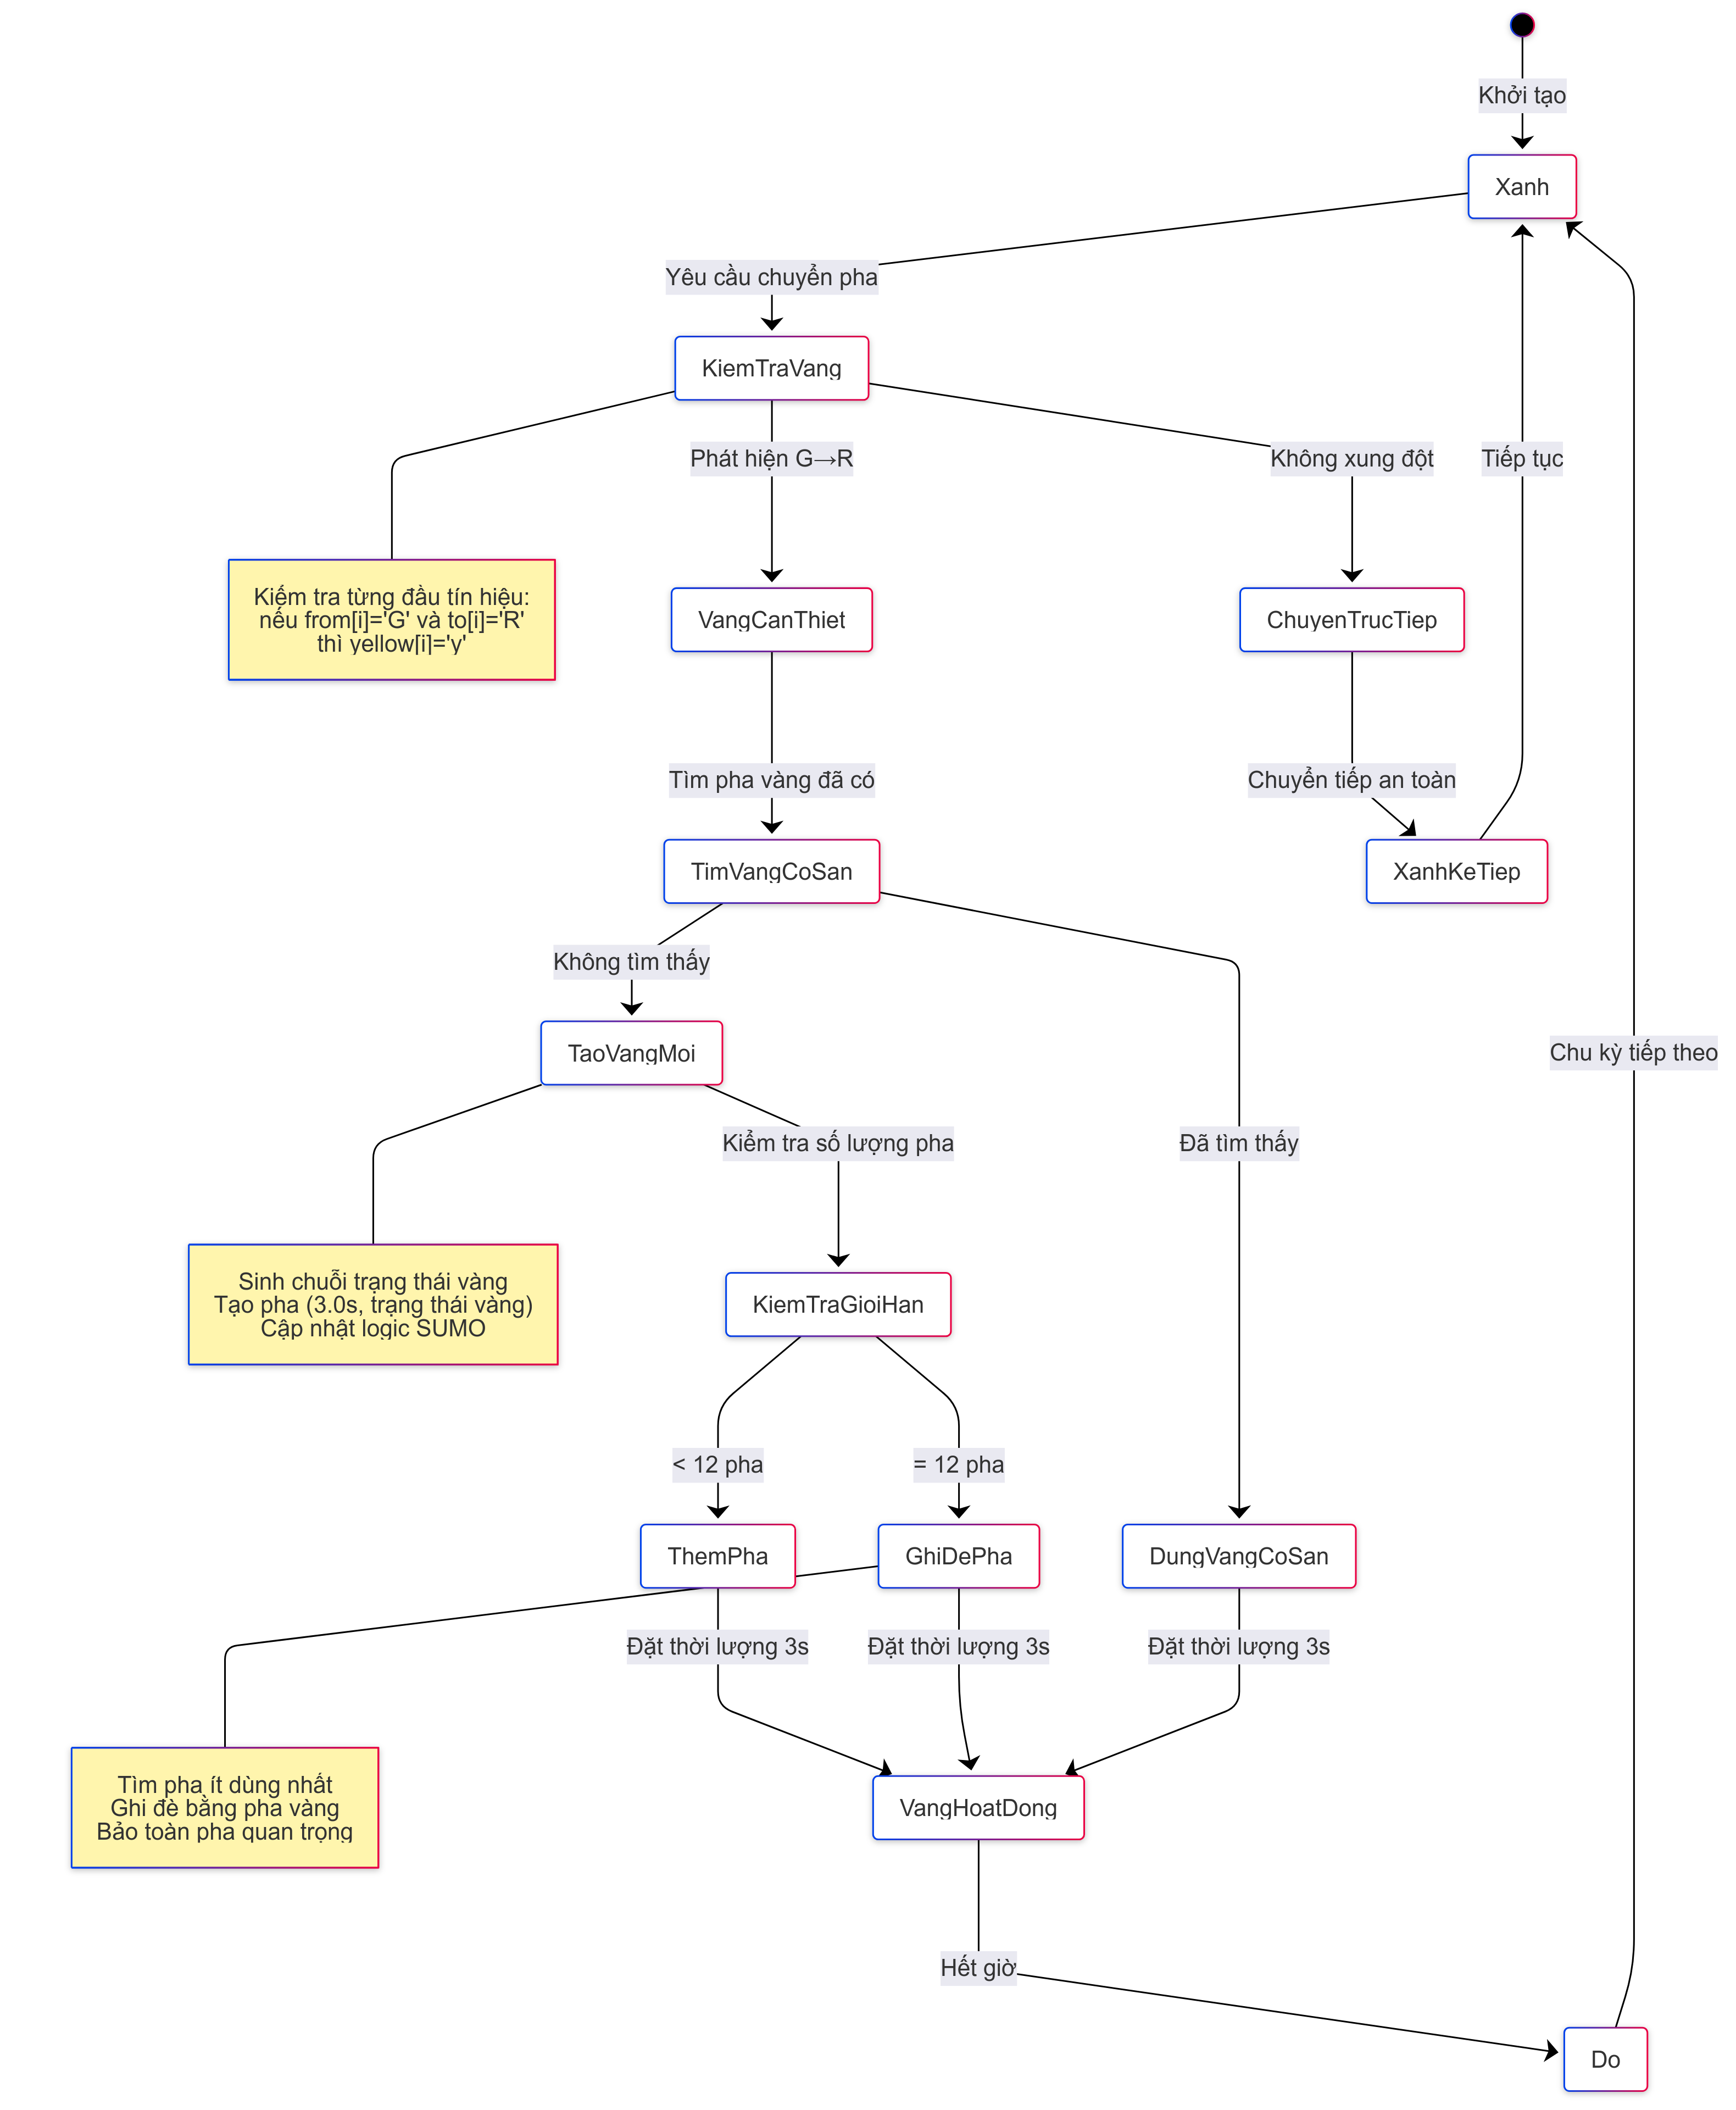
\includegraphics[width=0.75\linewidth]{Untitled diagram _ Mermaid Chart-2025-08-22-070255.png}
    \caption{Sơ đồ chuyển trạng thái với pha vàng tự động}
    \label{fig:placeholder}
\end{figure}

\subsection{Xử lý và ngăn chặn xung đột pha}

Hệ thống áp dụng nhiều cơ chế để phát hiện và ngăn chặn xung đột pha nguy hiểm.

\subsubsection{Ma trận phát hiện xung đột}

Tạo một bảng (ma trận) để kiểm tra và xác định các trường hợp xung đột giữa các luồng di chuyển (movement) trong các pha đèn giao thông.
\begin{lstlisting}[style=py, caption={Phase conflict detection}]
def detect_phase_conflicts(self, phase_state):
    controlled_links = traci.trafficlight.getControlledLinks(self.tls_id)
    conflicts = []
    
    for i, link_i in enumerate(controlled_links):
        if phase_state[i].upper() != 'G':
            continue
            
        for j, link_j in enumerate(controlled_links):
            if i == j or phase_state[j].upper() != 'G':
                continue
                
            # Check for conflicting movements
            if self.movements_conflict(link_i, link_j):
                conflicts.append((i, j))
                
    return conflicts
\end{lstlisting}

\subsubsection{Rate limiting for logic mutations}

Ngăn chặn rapid phase changes gây flicker:

\begin{lstlisting}[style=py, caption={Logic mutation rate limiting}]
def _can_mutate_logic(self):
    now = traci.simulation.getTime()
    cooldown = 2.0  # seconds
    
    if now - self._last_logic_mutation < cooldown:
        logger.info(f"[RATE-LIMIT] Skipping logic mutation; "
                   f"cooldown {cooldown}s")
        return False
        
    self._last_logic_mutation = now
    return True
\end{lstlisting}

\subsubsection{Quy tắc thiết lập pha đèn}

Hệ thống đảm bảo các quy tắc an toàn:

\begin{enumerate}
    \item \textbf{No all-red prevention}: Mọi pha phải có ít nhất một pha xanh
    \item \textbf{Conflicting movement check}: Không cho phép pha xanh đồng thời cho các hướng xung đột
    \item \textbf{Yellow transition requirement}: Bắt buộc yellow giữa các pha xanh xung đột
    \item \textbf{Maximum phase count}: Giới hạn 12 pha theo mặc định hệ thông giả lập SUMO
\end{enumerate}

\begin{figure}[htbp]
    \centering
    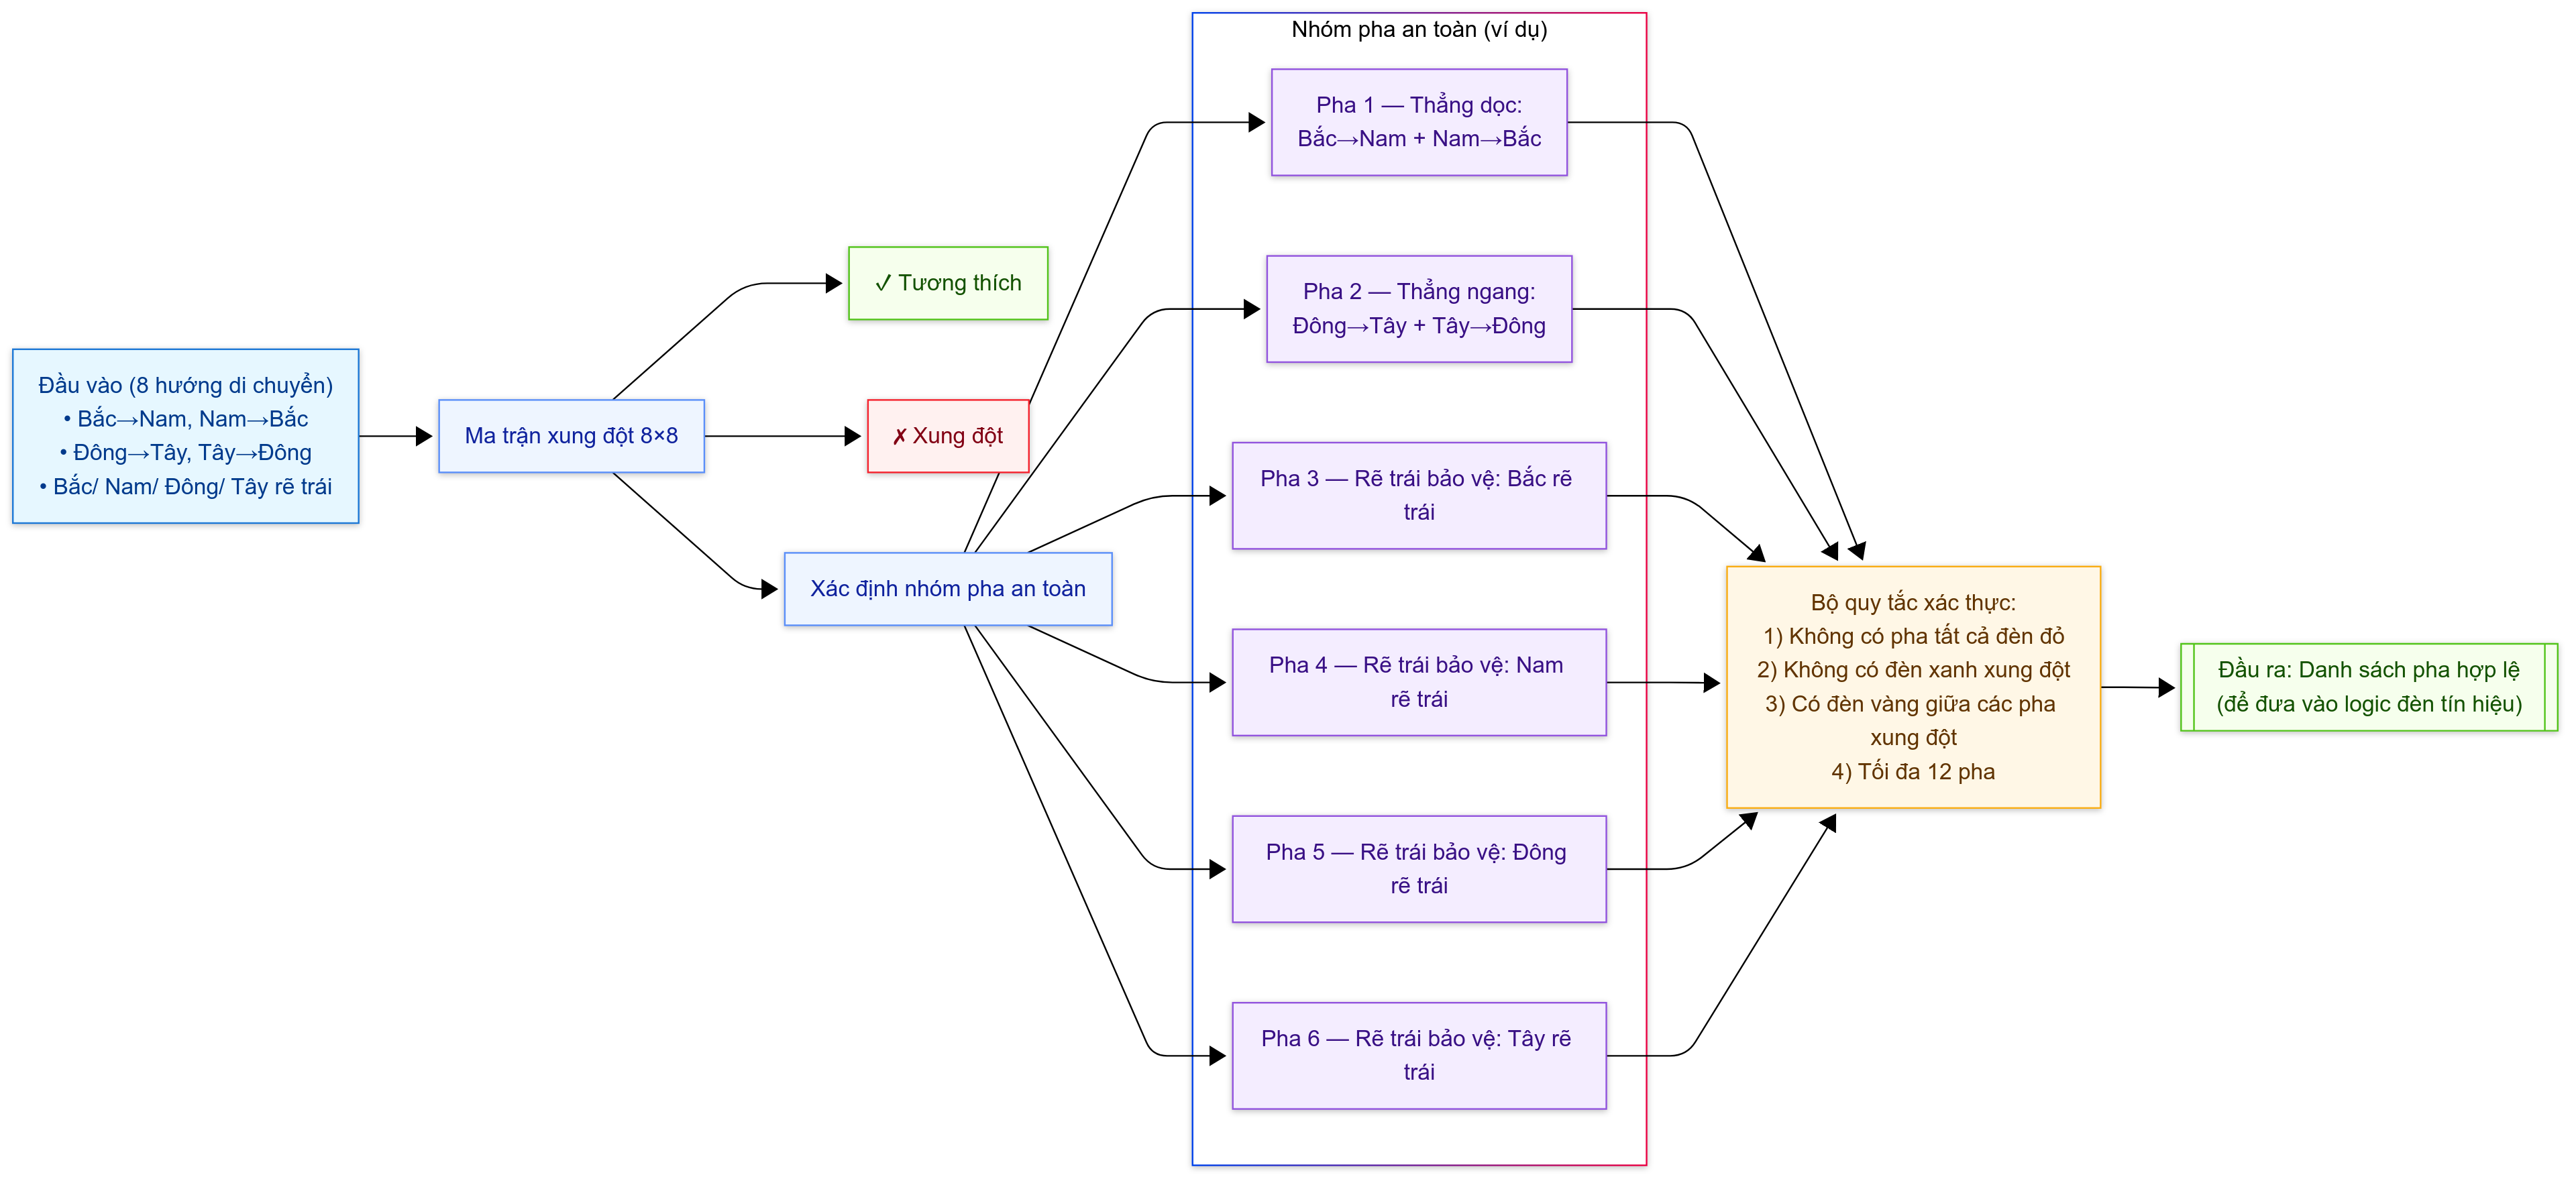
\includegraphics[width=1.0\linewidth]{Untitled diagram _ Mermaid Chart-2025-08-22-074409.png}
    \caption{Ma trận xung đột pha cho nút giao 4 hướng}
    \label{fig:conflict_matrix}
\end{figure}
\subsubsection{Cơ chế phục hồi}

Khi phát hiện vi phạm, hệ thống tự động khôi phục:

\begin{lstlisting}[style=py, caption={Automatic conflict resolution}]
def ensure_phases_have_green(self):
    logic = self._get_logic()
    changed = False
    
    for idx, phase in enumerate(logic.getPhases()):
        if 'G' not in phase.state:
            # Find first red and convert to green
            state_list = list(phase.state)
            for i, ch in enumerate(state_list):
                if ch == 'r':
                    state_list[i] = 'G'
                    break
                    
            new_state = ''.join(state_list)
            logger.info(f"[PATCH] Phase {idx} had no green, "
                       f"fixing: {phase.state} $\rightarrow$ {new_state}")
            self.overwrite_phase(idx, new_state, phase.duration)
            changed = True
            
    if changed:
        logger.info("[PATCH] All phases now have at least one green")
\end{lstlisting}

Hệ thống quản lý logic pha này đảm bảo hoạt động an toàn, hiệu quả và khả năng phục hồi cao cho điều khiển đèn giao thông trong mọi điều kiện vận hành.

\section{Điều chỉnh thời lượng pha động}

Trong hệ thống điều khiển pha thích nghi (APC), việc điều chỉnh thời lượng pha động là một thành phần cốt lõi giúp tối ưu hóa hiệu suất giao thông theo trạng thái thực tế tại nút giao. Quá trình này đảm bảo các pha đèn không bị cố định mà luôn được cập nhật linh hoạt dựa trên hàng chờ, tốc độ xe, thời gian chờ và các chỉ số reward tổng hợp. Dưới đây là mô tả chi tiết về các thuật toán và cơ chế vận hành:

\subsection{Thuật toán điều chỉnh delta-t}

Thuật toán điều chỉnh \(\Delta t\) là bước chuyển đổi phần thưởng (\(R\)) sang giá trị mở rộng hoặc rút ngắn thời lượng pha xanh. Cách tiếp cận này dựa trên sai lệch giữa reward thực tế và mục tiêu (\(R_{target}\)), kết hợp với làm mượt phi tuyến và phạt khi điều chỉnh quá lớn.

\paragraph{Công thức điều chỉnh thời lượng pha động:}
\[
\begin{aligned}
&\text{raw\_}\Delta t = \alpha \cdot (R - R_{\text{target}}) \\
&\Delta t = s \cdot \tanh\left(\frac{\text{raw\_}\Delta t}{s}\right) \\
&\Delta t^* = \mathrm{clip}\left(\Delta t,\ \Delta t_{\min},\ \Delta t_{\max}\right)
\end{aligned}
\]

Trong đó:
\begin{itemize}
    \item \(\alpha\): hệ số học, kiểm soát tốc độ điều chỉnh.
    \item \(s\): thang làm mượt (thường bằng giá trị điều chỉnh lớn nhất, ví dụ: 20).
    \item \(\mathrm{clip}\): hàm kẹp giá trị vào đoạn \([\Delta t_{\min}, \Delta t_{\max}]\) để tránh điều chỉnh quá mức.
\end{itemize}

Nếu giá trị \(\text{raw\_}\Delta t\) vượt quá ngưỡng an toàn \(\Delta t_{\text{large}}\), hệ thống áp dụng hình phạt:
\[
\text{penalty} = \max\left(0,\ |\text{raw\_}\Delta t| - \Delta t_{\text{large}}\right)
\]

\begin{figure}[H]
    \centering
    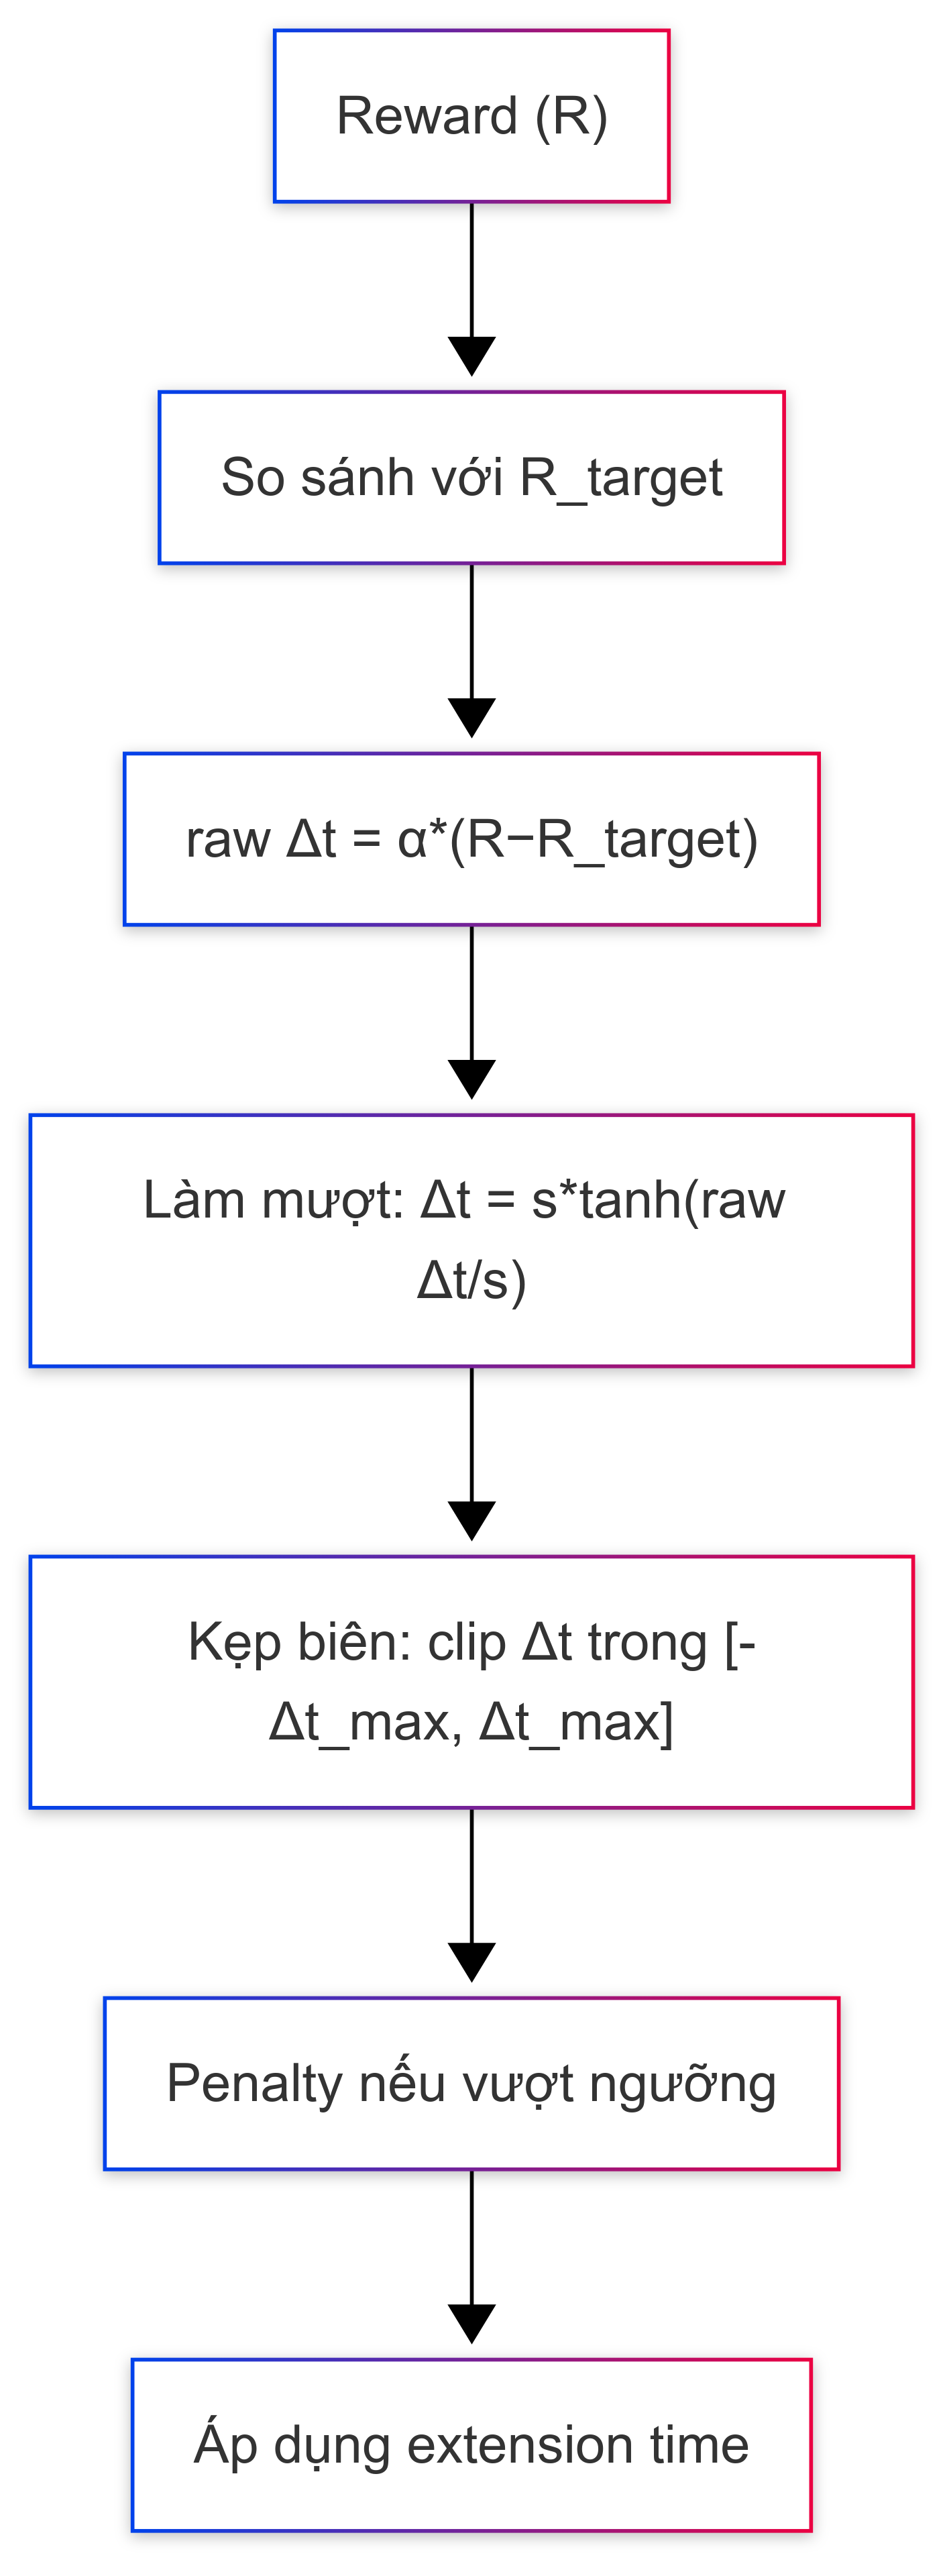
\includegraphics[width=0.55\linewidth]{Untitled diagram _ Mermaid Chart-2025-08-22-100758.png}
    \caption{Pipeline chuyển đổi phần thưởng thành điều chỉnh thời lượng pha}
    \label{fig:dynamic_timing_pipeline}
\end{figure}

\subsection{Cơ chế extension và cập nhật remaining time}

Sau khi xác định \(\Delta t\), hệ thống thực hiện hai bước chính để cập nhật thời lượng pha động:
\begin{enumerate}
    \item \textbf{Tính toán tổng thời lượng mong muốn cho pha hiện tại:} 
    \[
    \texttt{desired\_total} = \texttt{base\_duration} + \Delta t^*
    \]
    Giá trị này được kẹp vào khoảng \([\texttt{min\_green},\ \texttt{max\_green}]\) để đảm bảo không vượt quá giới hạn an toàn.
    
    \item \textbf{Cập nhật remaining time một cách chọn lọc:} 
    Chỉ thực hiện cập nhật khi độ chênh lệch giữa thời lượng mong muốn và giá trị hiện tại vượt ngưỡng buffer, nhằm tránh gửi lệnh điều khiển liên tục gây quá tải hệ thống.
\end{enumerate}

\begin{figure}[H]
    \centering
    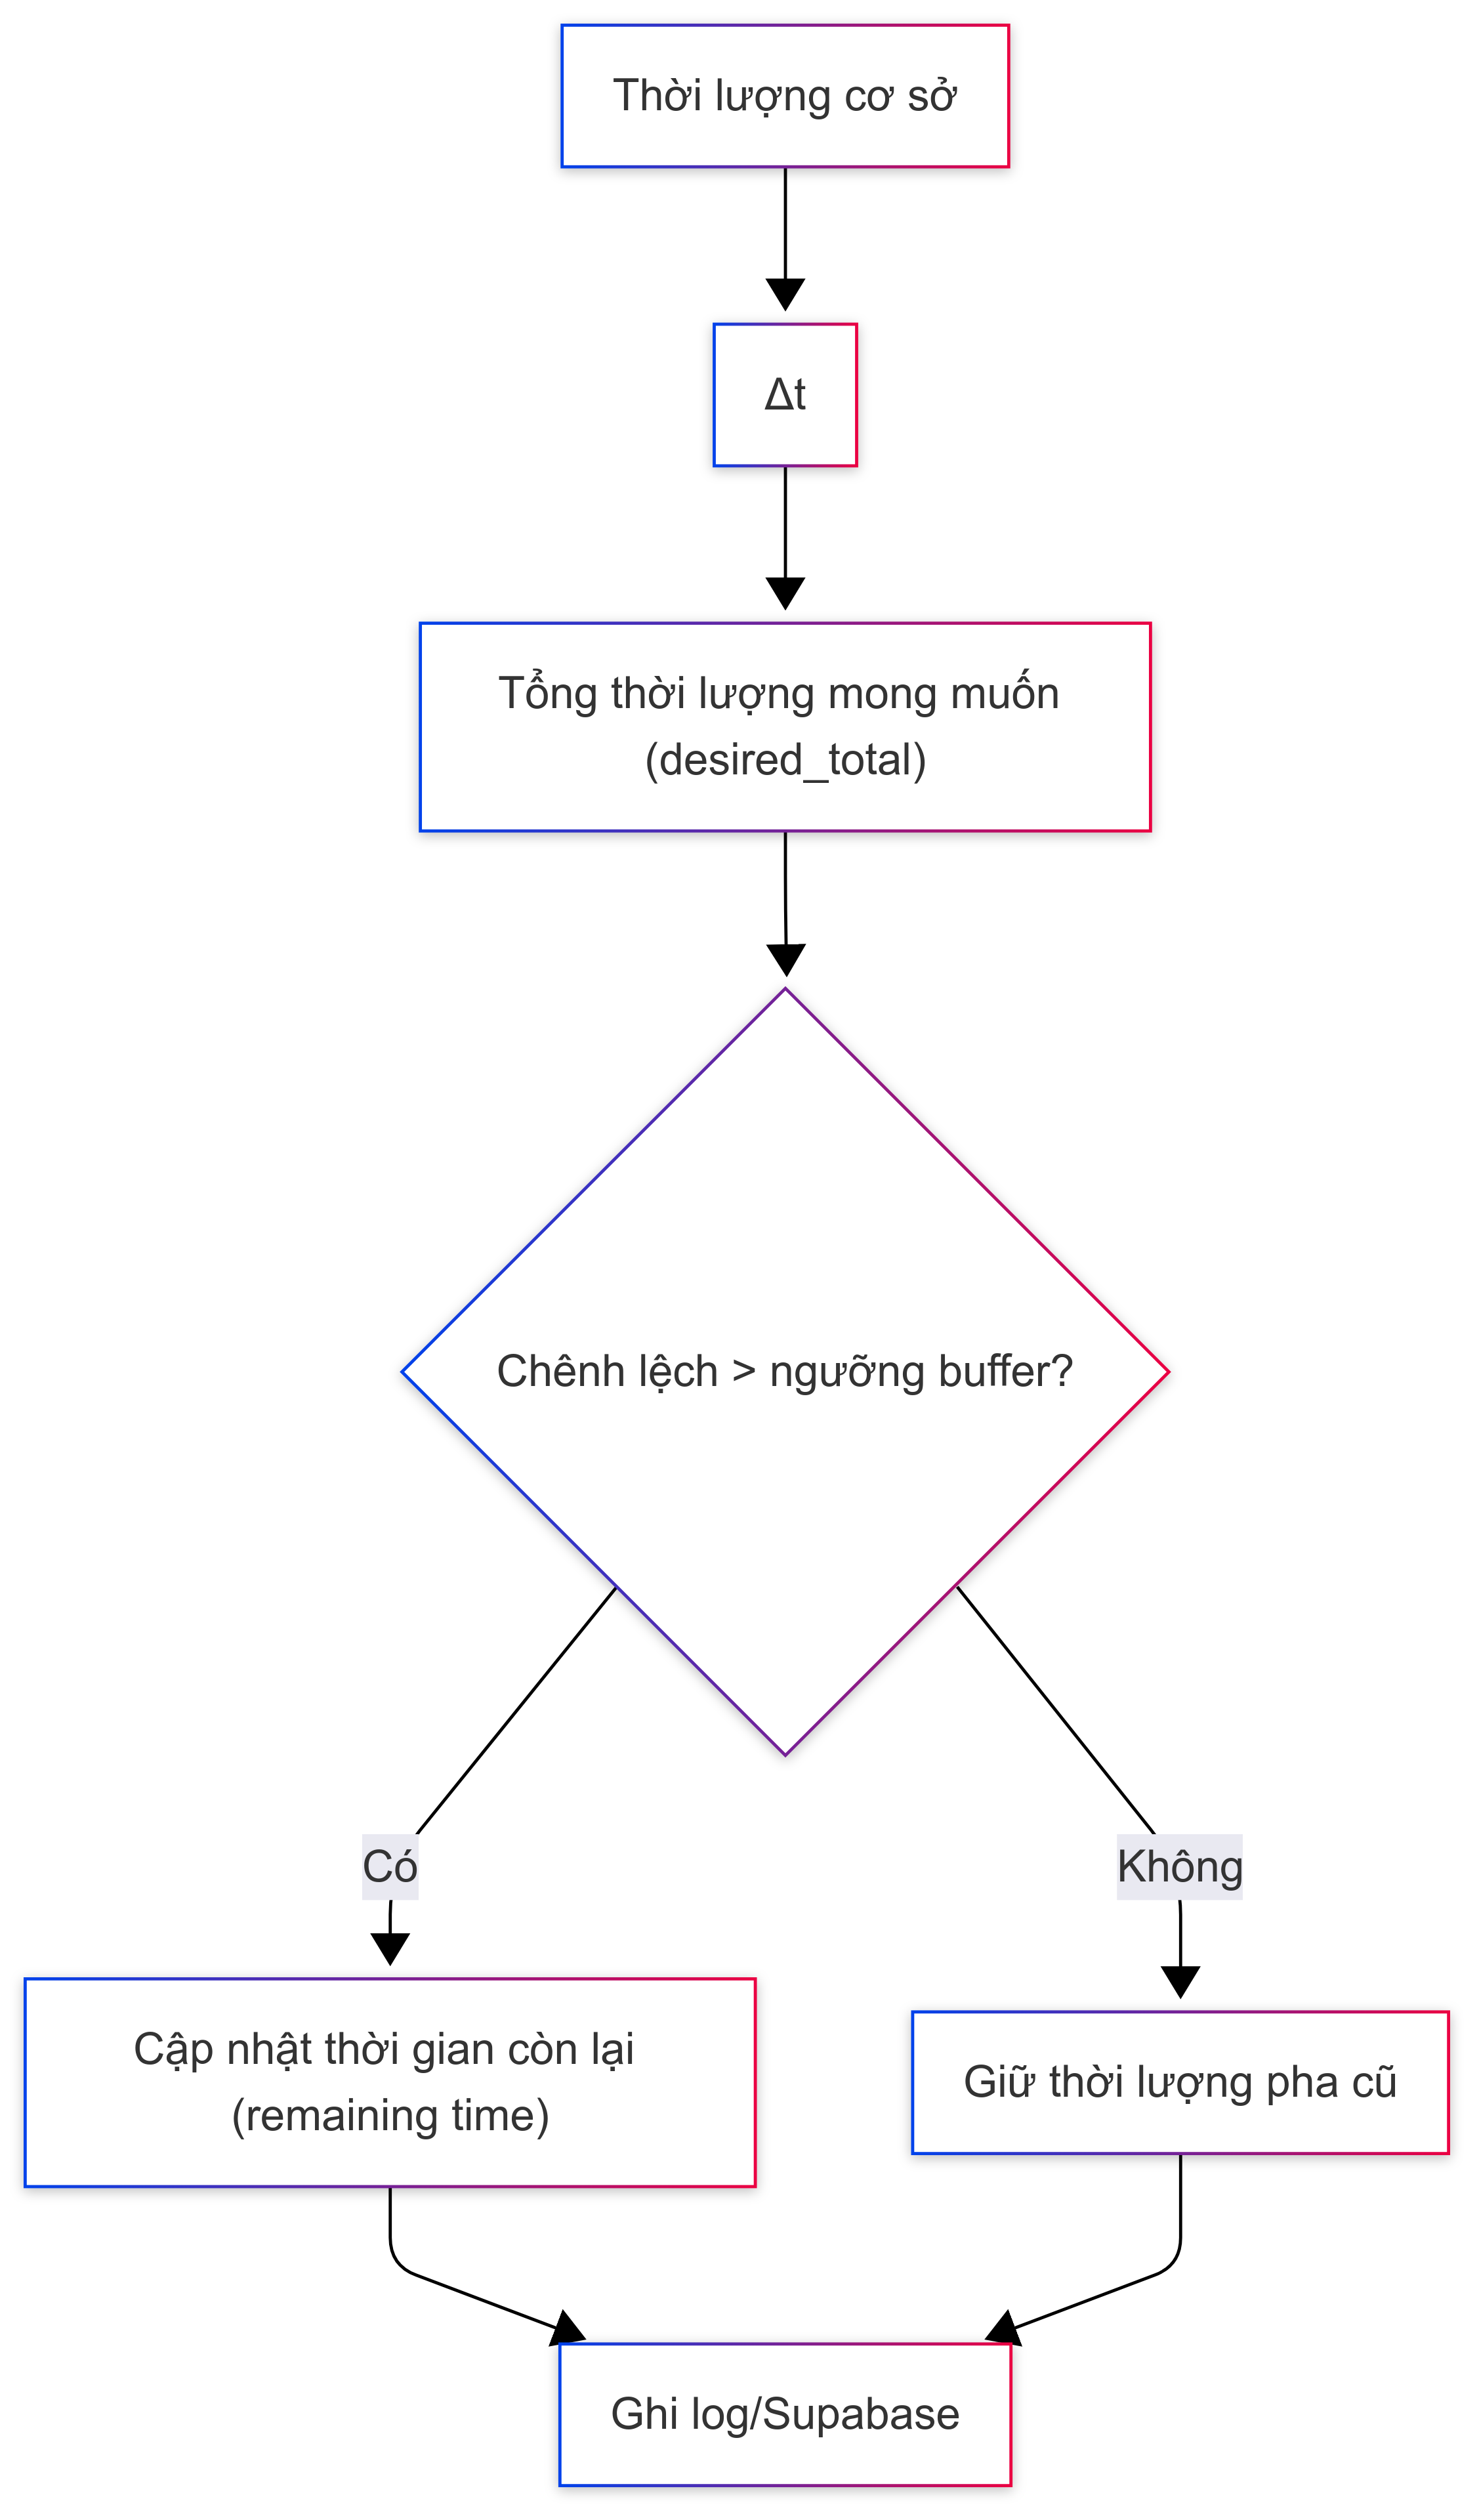
\includegraphics[width=0.5\textwidth, trim=0cm 2cm 0cm 0cm, clip]{Untitled diagram _ Mermaid Chart-2025-08-26-080816.png}
    \caption{Quy trình cập nhật remaining time cho pha động}
    \label{fig:extension_flow}
\end{figure}

Trong trường hợp nhu cầu giao thông rất thấp, phần mở rộng thời lượng (extension) sẽ bị giới hạn bởi tham số \texttt{low\_demand\_extend\_cap} để đảm bảo pha không kéo dài quá mức cần thiết. Quá trình này giúp trạng thái giữa bộ điều khiển APC và mô phỏng SUMO luôn được đồng bộ chính xác.
\subsection{Ràng buộc \texttt{min\_green} và \texttt{max\_green}}

Mọi thời lượng pha (\texttt{desired\_total}) đều bị ràng buộc trong khoảng \([\texttt{min\_green}, \texttt{max\_green}]\) để đảm bảo an toàn và công bằng phục vụ các hướng. Bộ điều khiển chặn chuyển pha nếu chưa đạt \texttt{min\_green}, trừ các trường hợp đặc biệt như phát hiện phương tiện khẩn cấp, protected left thực sự, hoặc starvation nghiêm trọng.

Ngoài ra, khi nhu cầu thực rất thấp, APC chỉ cho phép kéo đuôi pha ngắn để tăng tốc vòng lặp, giảm nguy cơ starvation cho các hướng khác.

\begin{figure}[H]
    \centering
    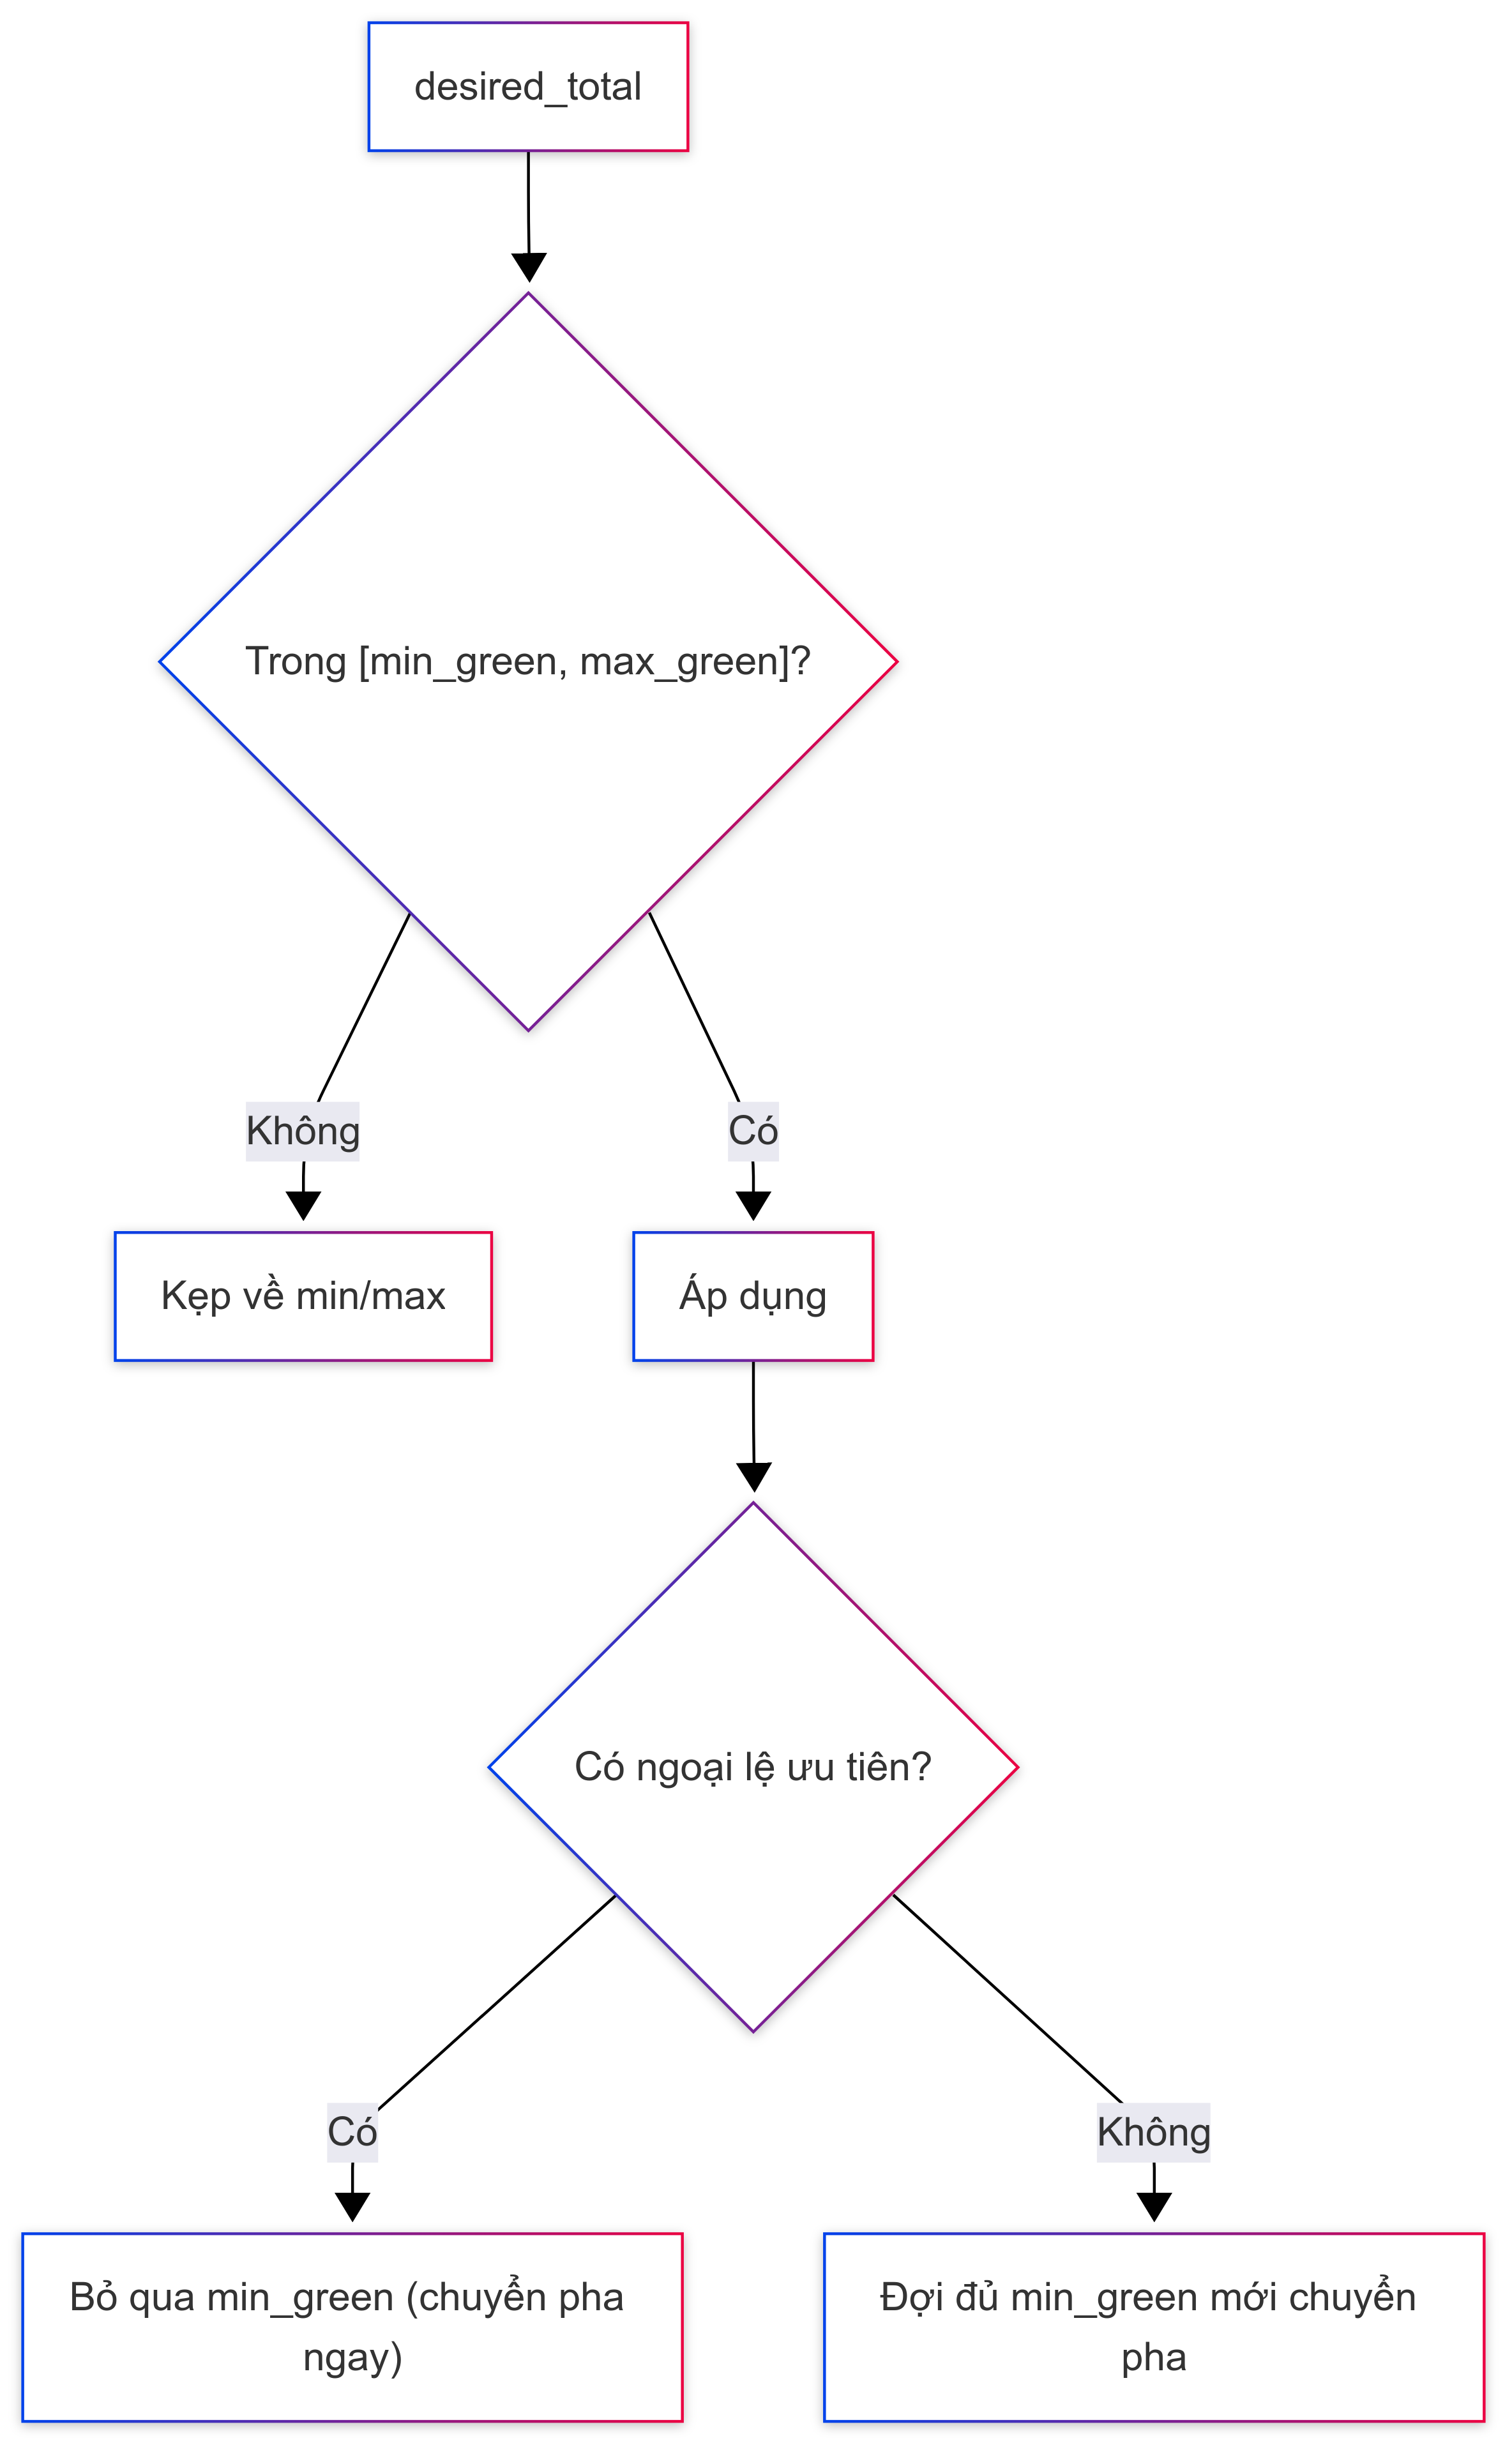
\includegraphics[width=0.5\linewidth]{Untitled diagram _ Mermaid Chart-2025-08-26-091434.png}
    \caption{Kiểm soát thời lượng pha với các ngưỡng ràng buộc}
    \label{fig:minmax_constraints}
\end{figure}
\subsection{Tính toán thời lượng tối ưu theo nhu cầu}

APC cung cấp các phương pháp heuristics để tính toán thời lượng pha tối ưu dựa trên trạng thái thực tế:
\begin{itemize}
    \item \textbf{Theo pha:} \texttt{calculate\_adaptive\_duration(phase\_idx)} dựa trên tổng hàng chờ của các lane xanh, pha trống sẽ rất ngắn còn pha bận rộn được mở rộng.
    \item \textbf{Theo làn:} \texttt{calculate\_optimal\_green\_time(lane\_id)} dựa trên thời gian giải tỏa hàng chờ và dung lượng downstream.
\end{itemize}

\begin{align*}
    &T_{\text{clear}} \approx 2.0 Q \\
    &T_{\text{downstream}} \approx 2.0 C_{\downarrow} \\
    &T^* = \min\left(\texttt{max\_green},\ \max\left(\texttt{min\_green},\ T_{\text{clear}},\ 2T_{\text{downstream}}\right) + k \lambda_{\text{arr}}\right)
\end{align*}

Trong đó:
\begin{itemize}
    \item $Q$: Tổng hàng chờ tại các làn được phục vụ.
    \item $C_{\downarrow}$: Dung lượng đoạn downstream.
    \item $\lambda_{\text{arr}}$: Tốc độ xe đến (arrival rate).
    \item $k$: Hệ số điều chỉnh nhỏ bổ sung cho nhu cầu sắp tới.
    \item \texttt{min\_green}, \texttt{max\_green}: Giới hạn thời lượng pha theo cấu hình.
\end{itemize}

Khi chọn pha tối ưu, APC sử dụng tổng hợp các yếu tố như hàng chờ lớn nhất, thời gian chờ, starvation, và áp lực downstream, kèm theo hysteresis để tránh dao động liên tục giữa các pha.


\begin{figure}
    \centering
    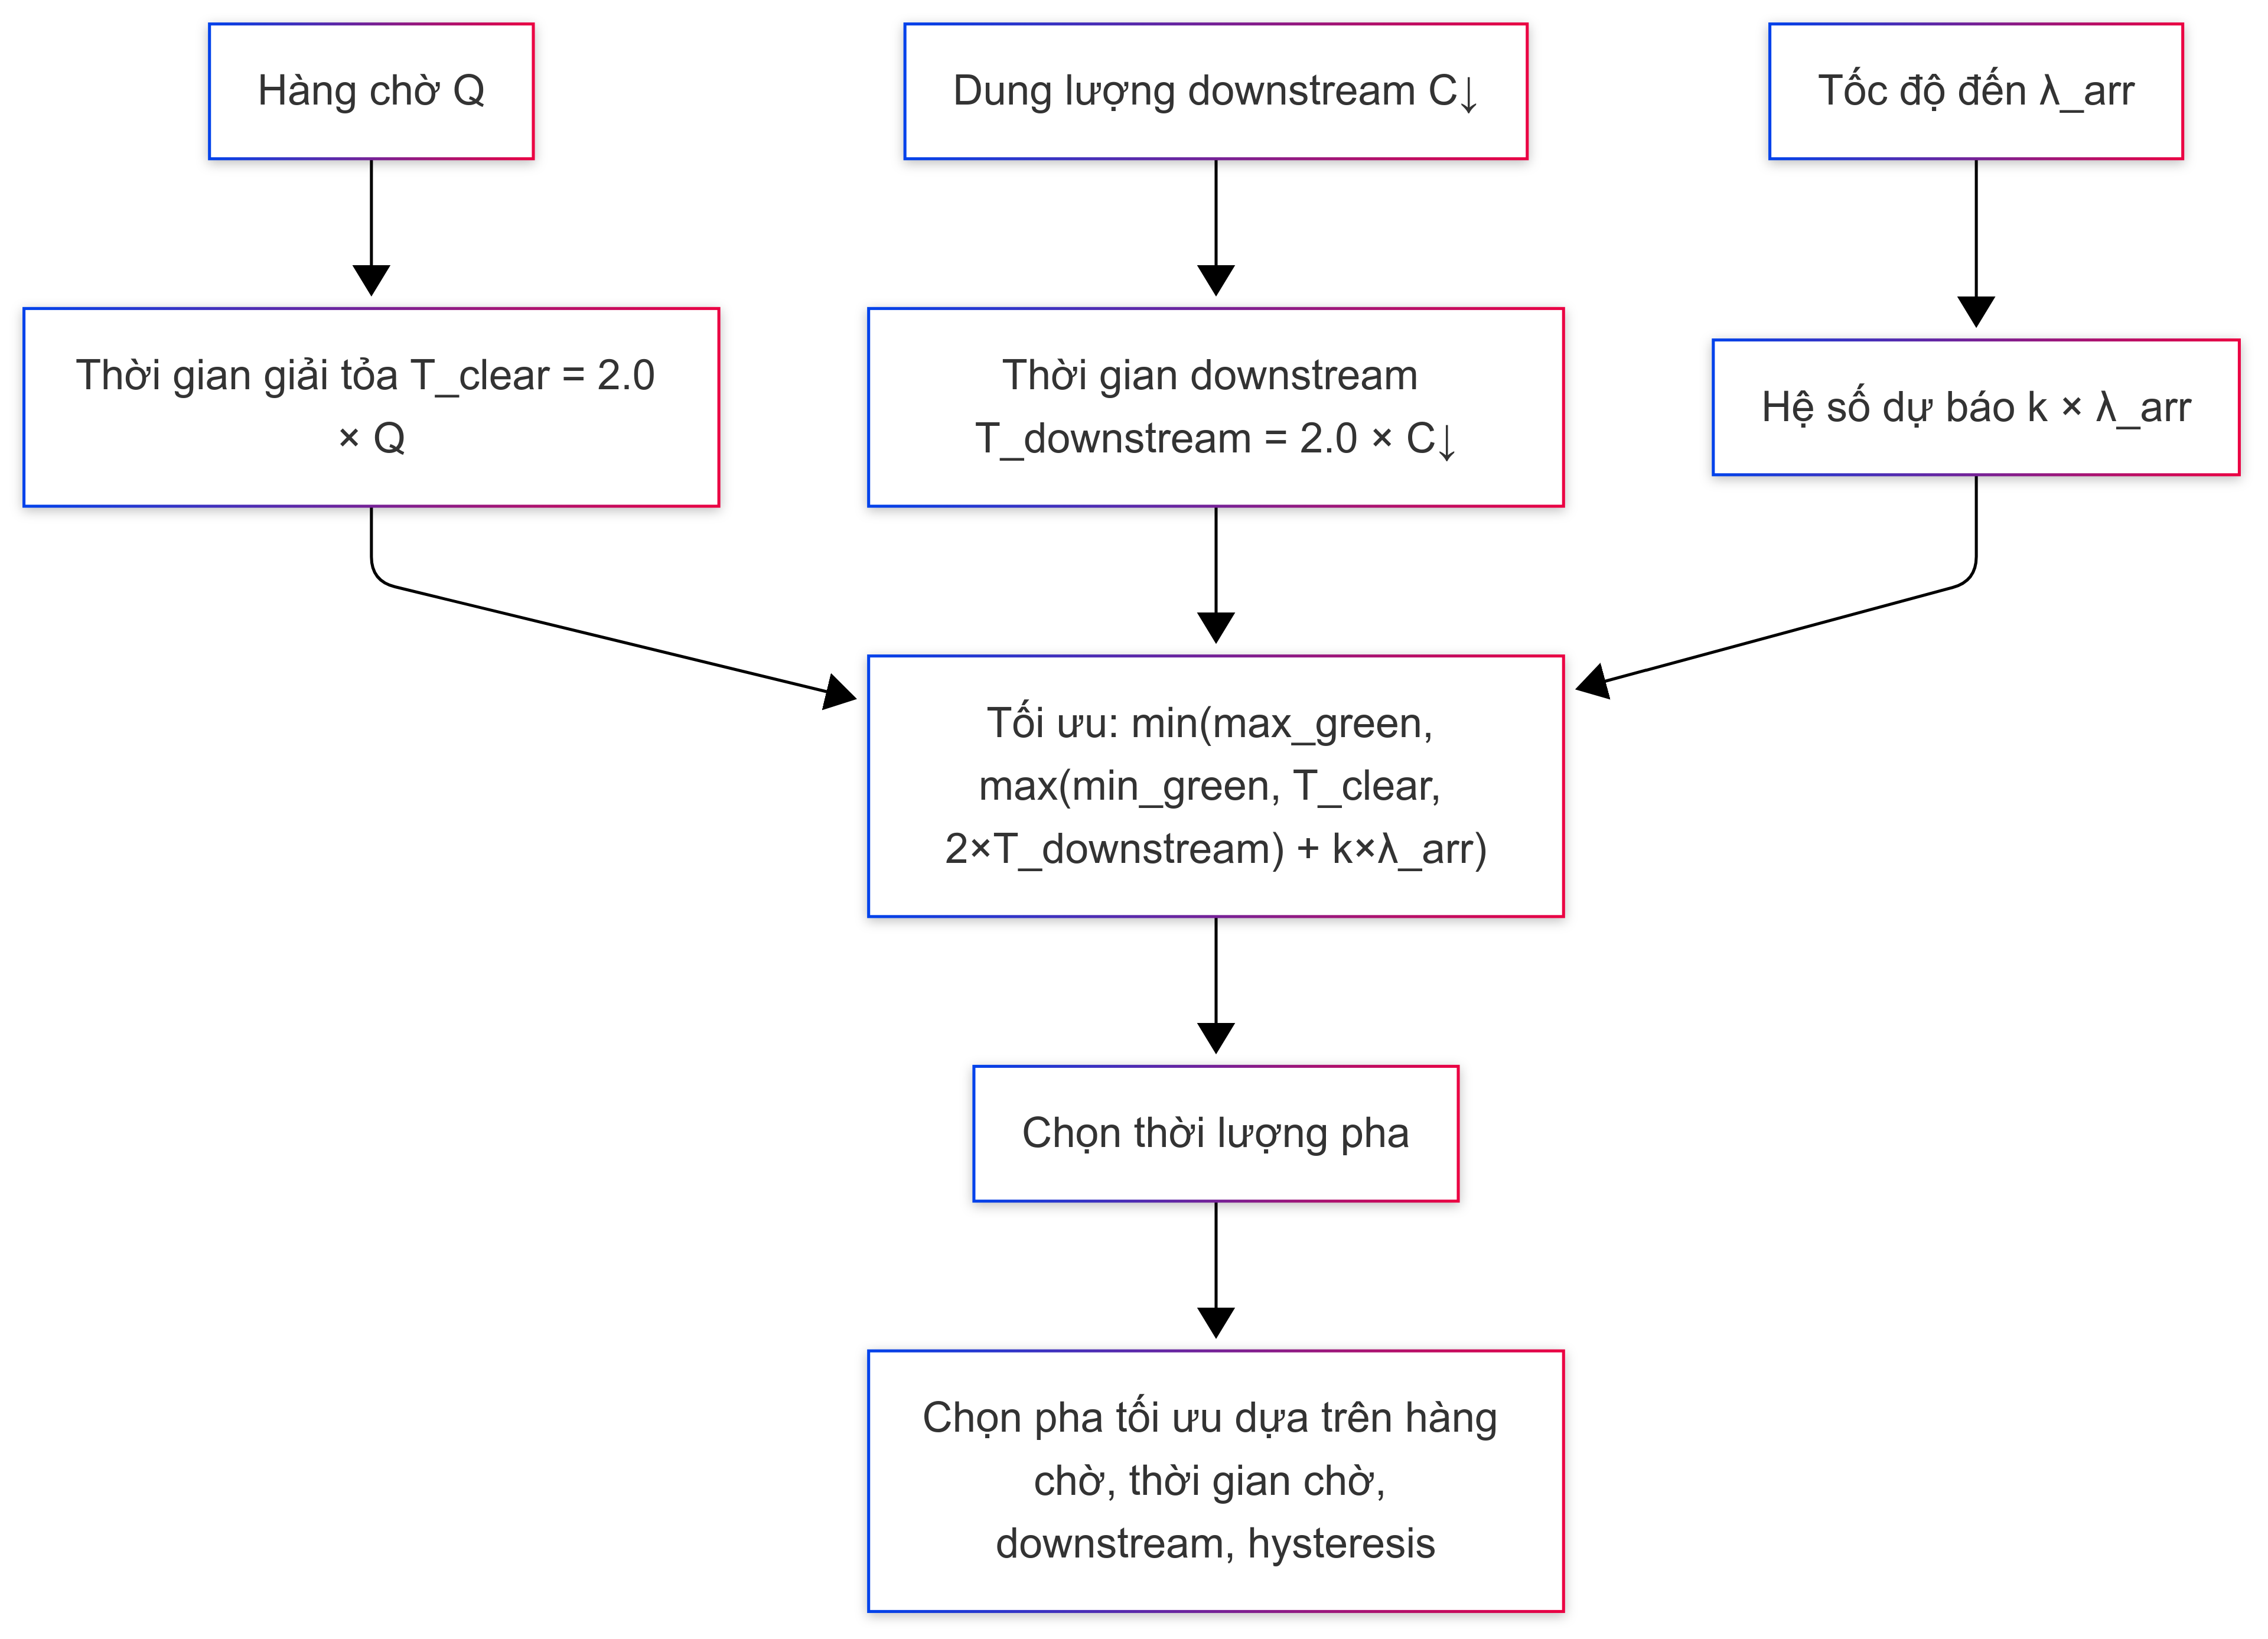
\includegraphics[width=0.75\linewidth]{Untitled diagram _ Mermaid Chart-2025-08-26-094113.png}
    \caption{Quy trình chọn thời lượng pha tối ưu dựa trên trạng thái giao thông}
    \label{fig:optimal_time_decision}
\end{figure}

% ... phần đầu giữ nguyên ...

\section{Hệ thống quản lý yêu cầu ưu tiên}

Hệ thống quản lý yêu cầu ưu tiên là thành phần cốt lõi giúp bộ điều khiển pha thích nghi (APC) xử lý hiệu quả các tình huống đặc biệt trong giao thông đô thị như xe khẩn cấp, starvation, tắc nghẽn cục bộ, hoặc các nhu cầu thay đổi pha do tình hình thực tế biến động.

\subsection{Cấu trúc hàng đợi yêu cầu phân cấp}

Hàng đợi yêu cầu (\texttt{pending\_requests}) được thiết kế dưới dạng danh sách ưu tiên (priority queue), trong đó mỗi yêu cầu có các trường thông tin:

\begin{itemize}
    \item \texttt{phase\_idx}: Chỉ số pha mục tiêu cần chuyển tới.
    \item \texttt{priority}: Giá trị số thể hiện mức độ ưu tiên (càng cao càng được xử lý trước).
    \item \texttt{priority\_type}: Loại yêu cầu, ví dụ \texttt{emergency}, \texttt{starvation}, \texttt{normal}, \texttt{congestion}.
    \item \texttt{extension\_duration}: Thời lượng pha mong muốn (nếu có).
    \item \texttt{timestamp}: Thời điểm phát sinh yêu cầu.
\end{itemize}

Các yêu cầu được sắp xếp giảm dần theo \texttt{priority}, nếu bằng nhau thì xét \texttt{timestamp} để đảm bảo yêu cầu đến trước được xử lý trước.

\begin{figure}[H]
    \centering
    \fbox{\parbox{0.7\textwidth}{\centering\vspace{3cm}
    \textit{[Diagram Placeholder: Sơ đồ cấu trúc hàng đợi yêu cầu phân cấp với các type priority và flow xử lý]}
    \vspace{3cm}}}
    \caption{Cấu trúc hàng đợi yêu cầu phân cấp cho APC}
    \label{fig:priority_queue_diagram}
\end{figure}

\subsection{Xử lý yêu cầu theo mức độ ưu tiên}

Quy trình xử lý yêu cầu được thực hiện định kỳ trong vòng lặp điều khiển. APC kiểm tra hàng đợi, ưu tiên các yêu cầu có \texttt{priority\_type} đặc biệt như:

\begin{itemize}
    \item \textbf{Emergency}: Xe cứu thương, cứu hỏa, cảnh sát — yêu cầu chuyển pha lập tức, vượt qua mọi ràng buộc thời gian xanh tối thiểu.
    \item \textbf{Critical starvation}: Hướng giao thông bị bỏ qua quá lâu, cần phục vụ để đảm bảo công bằng.
    \item \textbf{Congestion}: Tắc nghẽn cục bộ, cần điều chỉnh pha để giải tỏa hàng chờ.
    \item \textbf{Normal}: Các yêu cầu chuyển pha thông thường, phục vụ theo logic luân phiên.
\end{itemize}

Hệ thống sử dụng hàm \texttt{select\_best\_phase\_from\_requests()} để chọn yêu cầu có mức ưu tiên cao nhất. Các trường hợp đặc biệt như emergency sẽ được xử lý ngay cả khi chưa đủ thời gian xanh tối thiểu.

\begin{figure}[H]
    \centering
    \fbox{\parbox{0.8\textwidth}{\centering\vspace{3cm}
    \textit{[Flowchart Placeholder: Quy trình xử lý yêu cầu theo mức độ ưu tiên, từ kiểm tra emergency đến chuyển pha]}
    \vspace{3cm}}}
    \caption{Quy trình xử lý yêu cầu ưu tiên}
    \label{fig:priority_request_flow}
\end{figure}

\subsection{Cơ chế gom nhiều yêu cầu và xử lý hàng loạt}

Để tránh việc bỏ sót các yêu cầu đến liên tục, APC hỗ trợ cơ chế \textbf{stacked requests} — các yêu cầu chưa được phục vụ sẽ được giữ lại trong hàng đợi và xử lý theo lô (\textbf{batch processing}) khi pha hiện tại kết thúc hoặc có sự kiện khẩn cấp.

Cơ chế này đảm bảo:
\begin{itemize}
    \item Không bị mất yêu cầu quan trọng khi có nhiều yêu cầu cùng lúc.
    \item Xử lý theo nhóm, tăng hiệu quả chuyển pha và giảm overhead giao tiếp với SUMO.
    \item Các yêu cầu cùng loại (ví dụ nhiều xe khẩn cấp) được xử lý liên tục cho đến khi hết.
\end{itemize}

\begin{figure}[H]
    \centering
    \fbox{\parbox{0.7\textwidth}{\centering\vspace{2.5cm}
    \textit{[Diagram Placeholder: Sơ đồ stacked requests và batch processing trong hàng đợi APC]}
    \vspace{2.5cm}}}
    \caption{Cơ chế stacked requests và batch processing}
    \label{fig:stacked_requests_diagram}
\end{figure}

\subsection{Giải quyết xung đột giữa các yêu cầu}

Trong trường hợp có nhiều yêu cầu cùng lúc, hệ thống sử dụng các quy tắc:
\begin{enumerate}
    \item \textbf{Ưu tiên tuyệt đối cho emergency}: Bất kỳ yêu cầu khẩn cấp nào sẽ override mọi yêu cầu khác.
    \item \textbf{Starvation giải quyết sau emergency}: Nếu không có emergency thì chọn yêu cầu starvation có hàng chờ lớn nhất.
    \item \textbf{Congestion được ưu tiên tiếp theo}: Kích hoạt chế độ tắc nghẽn nếu phát hiện queue vượt ngưỡng.
    \item \textbf{Normal requests}: Chỉ xử lý khi không có yêu cầu đặc biệt nào tồn tại.
    \item \textbf{Batch conflict resolution}: Khi có nhiều yêu cầu cùng priority, thực hiện xử lý batch, chọn pha tốt nhất dựa trên scoring (hàng chờ, thời gian chờ, trạng thái downstream).
\end{enumerate}

Nếu xảy ra xung đột giữa các yêu cầu cùng loại, APC sẽ sử dụng hàm scoring để chọn hướng giao thông có nhu cầu cấp thiết nhất, đồng thời ghi log sự kiện để phục vụ phân tích sau này.

\begin{figure}[H]
    \centering
    \fbox{\parbox{0.8\textwidth}{\centering\vspace{2.5cm}
    \textit{[Flowchart Placeholder: Quy trình giải quyết xung đột giữa các yêu cầu, từ classification đến conflict resolution]}
    \vspace{2.5cm}}}
    \caption{Quy trình giải quyết xung đột yêu cầu ưu tiên}
    \label{fig:conflict_resolution_flow}
\end{figure}

\vspace{0.5cm}

\noindent\textbf{Tóm lại:} Hệ thống quản lý yêu cầu ưu tiên trong APC giúp đảm bảo mọi tình huống đặc biệt đều được xử lý kịp thời, tăng hiệu quả điều khiển đèn giao thông, giảm nguy cơ tắc nghẽn và cải thiện công bằng cho các hướng giao thông.

\section{Phát hiện và xử lý tắc nghẽn}

Việc phát hiện, đánh giá và xử lý tắc nghẽn là một trong những chức năng quan trọng nhất của bộ điều khiển giao thông thông minh. Dưới đây là các thành phần chính và các thuật toán được triển khai trong bộ điều khiển APC (AdaptivePhaseController) nhằm quản lý congestion, được rút trích từ mã nguồn.

\subsection{Thuật toán nhận diện tắc nghẽn giao thông}

Bộ điều khiển áp dụng thuật toán nhận diện nhiều dạng tắc nghẽn giao thông (như spillback, gridlock, congestion nghiêm trọng) bằng cách phân tích các chỉ số như độ dài hàng chờ, mức độ chiếm dụng làn đường, tốc độ xe, và trạng thái của các đoạn đường phía sau nút giao.
\begin{lstlisting}[style=py,caption={Hàm detect\_congestion\_patterns trong APC}]
def detect_congestion_patterns(self):
    congestion_types = {'spillback': False, 'gridlock': False,
                        'arterial': False, 'localized': False, 'critical': False}
    max_queue = 0
    total_severity = 0
    congested_lane_count = 0
    critical_lanes = []
    for lane_id in self.lane_ids:
        queue_length = traci.lane.getLastStepHaltingNumber(lane_id)
        lane_length = traci.lane.getLength(lane_id)
        occupancy = traci.lane.getLastStepOccupancy(lane_id)
        severity = self.calculate_congestion_severity(lane_id)
        max_queue = max(max_queue, queue_length)
        total_severity += severity
        if severity > 0.5:
            congested_lane_count += 1
        # Spillback detection
        if queue_length > 0.5 * (lane_length / 7.5):
            congestion_types['spillback'] = True
        # Gridlock detection
        if occupancy > 0.7:
            downstream_lanes = self.get_downstream_lanes(lane_id)
            blocked_count = sum(1 for dl in downstream_lanes
                                if traci.lane.getLastStepOccupancy(dl) > 0.5)
            if blocked_count > len(downstream_lanes) * 0.25:
                congestion_types['gridlock'] = True
    avg_severity = total_severity / max(len(self.lane_ids), 1)
    # Critical detection
    if (avg_severity > 0.6 or 
        congested_lane_count > len(self.lane_ids) * 0.35 or
        max_queue > 40):
        congestion_types['critical'] = True
    return congestion_types
\end{lstlisting}

\begin{figure}[H]
    \centering
    \fbox{\parbox{0.75\textwidth}{\centering\vspace{2.5cm}
    \textit{[Placeholder: Flowchart phát hiện các kiểu congestion pattern]}
    \vspace{2.5cm}}}
    \caption{Sơ đồ phát hiện các kiểu congestion pattern}
    \label{fig:congestion_patterns_diagram}
\end{figure}

\subsection{Tổng hợp nhiều yếu tố để xác định mức độ nghiêm trọng}
Chỉ số  mức độ nghiêm trọng (severity) được tổng hợp từ nhiều yếu tố: length queue, waiting time, speed drop, occupancy, downstream pressure. Công thức tính được triển khai như sau:

\begin{lstlisting}[style=py,caption={Hàm calculate\_congestion\_severity}]
def calculate_congestion_severity(self, lane_id):
    queue = traci.lane.getLastStepHaltingNumber(lane_id)
    wait_time = traci.lane.getWaitingTime(lane_id)
    speed = traci.lane.getLastStepMeanSpeed(lane_id)
    max_speed = traci.lane.getMaxSpeed(lane_id)
    occupancy = traci.lane.getLastStepOccupancy(lane_id)
    lane_length = traci.lane.getLength(lane_id)
    queue_ratio = (queue * 7.5) / max(lane_length, 1.0)
    severity = (
        0.40 * min(queue_ratio * 1.5, 1.0) +
        0.30 * min(wait_time / 60, 1.0) +
        0.15 * (1 - speed / max(max_speed, 0.1)) +
        0.10 * min(occupancy * 1.2, 1.0) +
        0.05 * min((queue / 20), 1.0)
    )
    if severity > 0.6:
        severity = min(1.0, severity * 1.3)
    if queue > 50:
        severity = max(severity, 0.85)
    return severity
\end{lstlisting}

\begin{figure}[H]
    \centering
    \fbox{\parbox{0.7\textwidth}{\centering\vspace{2.5cm}
    \textit{[Placeholder: Sơ đồ tổng hợp các yếu tố tính severity]}
    \vspace{2.5cm}}}
    \caption{Tổng hợp các yếu tố tính chỉ số severity}
    \label{fig:severity_factors_diagram}
\end{figure}

\subsection{Dự báo và phòng ngừa tắc nghẽn}
Việc dự báo tắc nghẽn được thực hiện bằng cách phân tích tốc độ xe đến và đi, tốc độ gia tăng hàng chờ, dung lượng của đoạn đường phía trước (downstream) và các đợt xe đến bất thường (arrival burst)
\begin{lstlisting}[style=py,caption={Hàm predict\_congestion}]
def predict_congestion(self, lane_id, horizon=30):
    current_queue = traci.lane.getLastStepHaltingNumber(lane_id)
    arrival_rate = self._calculate_arrival_rate(lane_id)
    departure_rate = self.calculate_departure_rate(lane_id)
    predicted_queue = current_queue + (arrival_rate - departure_rate) * float(horizon)
    lane_capacity = traci.lane.getLength(lane_id) / 7.5
    will_congest = predicted_queue > lane_capacity * 0.7
    if will_congest:
        self.request_preemptive_green(lane_id, priority='high')
    return will_congest
\end{lstlisting}

\begin{figure}[H]
    \centering
    \fbox{\parbox{0.7\textwidth}{\centering\vspace{2.5cm}
    \textit{[Placeholder: Sơ đồ pipeline dự báo và phòng ngừa tắc nghẽn]}
    \vspace{2.5cm}}}
    \caption{Pipeline dự báo tắc nghẽn và quyết định phòng ngừa}
    \label{fig:congestion_forecast_diagram}
\end{figure}

\subsection{Kích hoạt chế độ tắc nghẽn}

Khi phát hiện tắc nghẽn nghiêm trọng, hệ thống chuyển sang chế độ tắc nghẽn với các tham số điều khiển đặc biệt:

\begin{lstlisting}[style=py,caption={Hàm activate\_congestion\_mode}]
def activate_congestion_mode(self):
    self.logger.info(f"[CONGESTION MODE] Activated for {self.tls_id}")
    self.min_green = 15
    self.max_green = 90
    self.alpha = 1.5
    self.weights = np.array([0.5, 0.1, 0.3, 0.1])
    self.protected_left_min_queue = 10
    self.serve_empty_greens = False
\end{lstlisting}

\begin{figure}[H]
    \centering
    \fbox{\parbox{0.65\textwidth}{\centering\vspace{2.5cm}
    \textit{[Placeholder: Flowchart kích hoạt và kiểm soát congestion mode]}
    \vspace{2.5cm}}}
    \caption{Quy trình kích hoạt và kiểm soát congestion mode}
    \label{fig:congestion_mode_diagram}
\end{figure}

\section{Quản lý rẽ trái bảo vệ thông minh}

\subsection{Phát hiện blocked left turn với xung đột}

Bộ điều khiển kiểm tra các làn rẽ trái, xác định blockage bằng phân tích queue, tốc độ, xung đột và downstream:

\begin{lstlisting}[style=py,caption={Hàm detect\_blocked\_left\_turn\_with\_conflict}]
def detect_blocked_left_turn_with_conflict(self):
    controlled_lanes = traci.trafficlight.getControlledLanes(self.tls_id)
    for lane_id in controlled_lanes:
        links = traci.lane.getLinks(lane_id)
        is_left = any(len(link) > 6 and link[6] == 'l' for link in links)
        if not is_left:
            continue
        queue, waiting_time, mean_speed, density = self.get_lane_stats(lane_id)
        vehicles = traci.lane.getLastStepVehicleIDs(lane_id)
        if not vehicles or queue < self.protected_left_min_queue:
            continue
        speed_blocked = mean_speed < 2.0
        density_blocked = density > 0.08
        if speed_blocked or density_blocked:
            conflicting_lanes = self.get_conflicting_straight_lanes(lane_id)
            has_conflict = any(
                (self.is_lane_green(conf_lane) and traci.lane.getLastStepVehicleNumber(conf_lane) > 0)
                for conf_lane in conflicting_lanes
            )
            if has_conflict:
                self.blocked_left_memory[lane_id] = min(self.blocked_left_memory.get(lane_id, 0) + 1, 100)
                return lane_id, True
    self._decay_blocked_memory()
    return None, False
\end{lstlisting}

\begin{figure}[H]
    \centering
    \fbox{\parbox{0.7\textwidth}{\centering\vspace{2.5cm}
    \textit{[Placeholder: Sơ đồ phát hiện blocked left turn và kiểm tra xung đột]}
    \vspace{2.5cm}}}
    \caption{Quy trình phát hiện và xác nhận blocked left turn}
    \label{fig:blocked_left_detection_diagram}
\end{figure}

\subsection{Tạo pha protected left động}

Khi phát hiện blocked left turn, APC sẽ tạo hoặc kích hoạt protected left phase phục vụ rẽ trái riêng biệt:

\begin{lstlisting}[style=py,caption={Hàm create\_protected\_left\_phase\_for\_lane}]
def create_protected_left_phase_for_lane(self, left_lane):
    controlled_links = traci.trafficlight.getControlledLinks(self.tls_id)
    left_link_indices = [i for i, link in enumerate(controlled_links) if link[0][0] == left_lane]
    protected_state = ''.join('G' if i in left_link_indices else 'r' for i in range(len(controlled_links)))
    # Check for existing identical phase
    for idx, phase in enumerate(self._get_logic().phases):
        if phase.state == protected_state:
            return self._safe_phase_index(idx, force_reload=True)
    # Otherwise, append new phase
    green_phase = traci.trafficlight.Phase(self.max_green, protected_state)
    yellow_state = ''.join('y' if i in left_link_indices else 'r' for i in range(len(controlled_links)))
    yellow_phase = traci.trafficlight.Phase(3, yellow_state)
    phases = list(self._get_logic().getPhases()) + [green_phase, yellow_phase]
    new_logic = traci.trafficlight.Logic(self._get_logic().programID, self._get_logic().type, len(phases) - 2, phases)
    traci.trafficlight.setCompleteRedYellowGreenDefinition(self.tls_id, new_logic)
    self._invalidate_logic_cache()
    return self._safe_phase_index(len(phases) - 2, force_reload=True)
\end{lstlisting}

\begin{figure}[H]
    \centering
    \fbox{\parbox{0.7\textwidth}{\centering\vspace{2.5cm}
    \textit{[Placeholder: Flowchart tạo hoặc kích hoạt pha protected left động]}
    \vspace{2.5cm}}}
    \caption{Quy trình tạo/kích hoạt pha protected left động}
    \label{fig:protected_left_phase_diagram}
\end{figure}

\subsection{Cơ chế memory và guard deadline}

Để tránh việc kích hoạt quá lâu, APC sử dụng bộ nhớ trạng thái blocked và guard deadline:

\begin{lstlisting}[style=py,caption={Cơ chế memory và guard deadline}]
self.blocked_left_memory[lane_id] = min(self.blocked_left_memory.get(lane_id, 0) + 1, 100)
self.blocked_focus_lane = lane_id
self.blocked_guard_deadline = current_time + max(2*self.min_green, 15.0)
\end{lstlisting}

\begin{figure}[H]
    \centering
    \fbox{\parbox{0.7\textwidth}{\centering\vspace{2.5cm}
    \textit{[Placeholder: Sơ đồ memory/guard deadline cho quản lý protected left]}
    \vspace{2.5cm}}}
    \caption{Cơ chế memory và guard deadline cho pha rẽ trái bảo vệ}
    \label{fig:protected_left_memory_diagram}
\end{figure}

\subsection{Tối ưu thời lượng protected left phase}

Thời lượng protected left phase được tối ưu dựa trên queue, waiting time, downstream và max\_green:

\begin{lstlisting}[style=py,caption={Tối ưu thời lượng protected left phase}]
queue = traci.lane.getLastStepHaltingNumber(left_lane)
wait = traci.lane.getWaitingTime(left_lane)
green_duration = min(self.max_green, max(self.min_green, queue * 2 + wait * 0.1))
self.set_phase_from_API(phase_idx, requested_duration=green_duration)
\end{lstlisting}

\begin{figure}[H]
    \centering
    \fbox{\parbox{0.7\textwidth}{\centering\vspace{2.5cm}
    \textit{[Placeholder: Flowchart tối ưu thời lượng protected left phase]}
    \vspace{2.5cm}}}
    \caption{Quy trình tối ưu thời lượng protected left phase}
    \label{fig:protected_left_duration_diagram}
\end{figure}

\vspace{0.5cm}


% ================================
% Phụ lục: Chi tiết thuật toán bộ điều khiển thông minh
% ================================

\section{Xử lý tình huống khẩn cấp}

\subsection{Phát hiện phương tiện ưu tiên}

Trong môi trường giao thông đô thị, các phương tiện ưu tiên (ví dụ: xe cứu thương, xe cứu hỏa, xe công vụ) cần được xử lý đặc biệt để đảm bảo thời gian di chuyển nhanh nhất có thể. Bộ điều khiển khai thác dữ liệu mô phỏng từ SUMO, trong đó mỗi phương tiện được gán một \textit{loại} (vehicle type). Các loại được gắn nhãn là \texttt{emergency} hoặc \texttt{authority} sẽ tự động kích hoạt chế độ ưu tiên.

\begin{lstlisting}[style=py,caption={Thuật toán phát hiện xe ưu tiên}]
def check_special_events(self):
    for lane_id in self.lane_ids:
        for vid in traci.lane.getLastStepVehicleIDs(lane_id):
            v_type = traci.vehicle.getTypeID(vid)
            if 'emergency' in v_type or 'priority' in v_type:
                self._log_apc_event({
                    "action": "emergency_vehicle",
                    "lane_id": lane_id,
                    "vehicle_id": vid,
                    "vehicle_type": v_type
                })
                return 'emergency_vehicle', lane_id
    return None, None
\end{lstlisting}

\begin{figure}[H]
    \centering
    \fbox{\parbox{0.7\textwidth}{\centering\vspace{2.5cm}
    \textit{[Sơ đồ phát hiện phương tiện ưu tiên và kích hoạt chế độ ưu tiên]}}}
    \caption{Quy trình phát hiện và xử lý phương tiện ưu tiên}
\end{figure}

\subsection{Emergency rebalancing khi mất cân bằng lưu lượng}

Trong một số tình huống, hệ thống có thể phát hiện trạng thái \textit{lane imbalance} nghiêm trọng, tức là nhiều làn trống trong khi một số làn lại ùn tắc kéo dài. Để ứng phó, bộ điều khiển tạm thời ưu tiên phục vụ các làn có mức tắc nghẽn cao nhất bằng cách điều chỉnh pha tín hiệu.

\begin{lstlisting}[style=py,caption={Cơ chế emergency rebalancing khi lane imbalance}]
def emergency_rebalance_phases(self):
    empty_lanes = []
    critical_lanes = []
    for lane in self.lane_ids:
        veh_count = traci.lane.getLastStepVehicleNumber(lane)
        queue = traci.lane.getLastStepHaltingNumber(lane)
        if veh_count == 0:
            empty_lanes.append(lane)
        elif queue > 10:
            critical_lanes.append((lane, queue))
    if critical_lanes and len(empty_lanes) > len(self.lane_ids) * 0.5:
        worst_lane, worst_queue = max(critical_lanes, key=lambda x: x[1])
        phase = self.find_or_create_phase_for_lane(worst_lane)
        if phase is not None:
            duration = min(60, max(30, worst_queue * 2))
            self.set_phase_from_API(phase, requested_duration=duration)
            return True
    return False
\end{lstlisting}

\begin{figure}[H]
    \centering
    \fbox{\parbox{0.7\textwidth}{\centering\vspace{2.5cm}
    \textit{[Quy trình phát hiện và xử lý mất cân bằng lưu lượng]}}}
    \caption{Sơ đồ emergency rebalancing khi xảy ra lane imbalance}
\end{figure}

\subsection{Xử lý starvation và ùn tắc nghiêm trọng}

Bên cạnh việc cân bằng lưu lượng, hệ thống còn giám sát hiện tượng \textit{starvation}, tức một số làn không được phục vụ trong thời gian dài. Nếu thời gian chờ của một làn vượt ngưỡng định trước, pha phục vụ sẽ được kích hoạt để tránh tình trạng xe không được giải tỏa. Đối với các trường hợp \textit{critical congestion}, hệ thống có thể chủ động kéo dài hoặc ưu tiên pha.

\begin{lstlisting}[style=py,caption={Thuật toán xử lý starvation và critical congestion}]
for lane in self.lane_ids:
    time_since_served = now - self.last_served_time.get(lane, 0)
    if time_since_served > 180 and traci.lane.getLastStepHaltingNumber(lane) > 0:
        phase = self.find_or_create_phase_for_lane(lane)
        if phase is not None:
            self.set_phase_from_API(phase, requested_duration=45)
            self.last_served_time[lane] = now
\end{lstlisting}

\begin{figure}[H]
    \centering
    \fbox{\parbox{0.7\textwidth}{\centering\vspace{2.5cm}
    \textit{[Quy trình phát hiện starvation và xử lý congestion]}}}
    \caption{Cơ chế xử lý starvation và ùn tắc nghiêm trọng}
\end{figure}

\subsection{Cơ chế cooldown và chống nhấp nháy pha (flicker)}

Một thách thức khác là hiện tượng chuyển pha quá nhanh (\textit{flicker}), gây rối loạn dòng giao thông. Bộ điều khiển áp dụng bộ đếm \textit{cooldown} kết hợp với logic so sánh pha trước/sau nhằm ngăn chặn các thay đổi tín hiệu liên tục, chỉ cho phép chuyển pha khi đủ thời gian an toàn đã trôi qua.

\begin{lstlisting}[style=py,caption={Cơ chế cooldown và ngăn chặn flicker}]
if self.last_phase_idx == new_phase_idx:
    logger.info(f"[PHASE SWITCH BLOCKED] Flicker prevention triggered for {self.tls_id}")
    return False
if now - getattr(self, "_last_logic_mutation", -1e9) < LOGIC_MUTATION_COOLDOWN_S:
    logger.info(f"[RATE-LIMIT] Skipping logic mutation; cooldown active")
    return False
\end{lstlisting}

\begin{figure}[H]
    \centering
    \fbox{\parbox{0.7\textwidth}{\centering\vspace{2.5cm}
    \textit{[Sơ đồ cơ chế cooldown và chống flicker]}}}
    \caption{Quy trình cooldown để ngăn chặn hiện tượng flicker pha}
\end{figure}
